\documentclass[12pt]{book}
\usepackage{geometry}
\geometry{letterpaper, left=22.5mm, right=22.5mm, top=30mm, bottom=30mm}
\geometry{letterpaper}
\usepackage{amsmath}
\usepackage{amssymb}
\usepackage{enumitem}
\usepackage{fancyhdr}
\usepackage{framed}
\usepackage{tikz}
\usepackage{mathpazo}
%\usepackage{charter}
%\usepackage{newcent}
\usepackage{indentfirst}
\usepackage{booktabs}
\usepackage{graphicx}
\usepackage{float}
\usepackage{makecell}
\usepackage{xcolor}
\usepackage{mdframed}
\usetikzlibrary{trees}
\pagestyle{fancy}
\usepackage{amsthm}
\theoremstyle{definition}
\newtheorem{definition}{Definition}[section]
\theoremstyle{property}
\newtheorem{property}{Property}[section]
\theoremstyle{assumption}
\newtheorem{assumption}{Assumption}[section]
\theoremstyle{example}
\newtheorem{example}{Example}[section]
\theoremstyle{comment}
\newtheorem{comment}{Comment}[section]
\newtheorem{theorem}{Theorem}[section]
\newtheorem{corollary}{Corollary}[theorem]
\newtheorem{lemma}[theorem]{Lemma}
\usepackage{lastpage}
\usepackage{wrapfig}
\usepackage{hyperref}
\usepackage{subcaption}
\usepackage{setspace}
\hypersetup{
colorlinks=true,
linkcolor=black,
filecolor=green, 
urlcolor=blue,
}
\newcommand{\ROM}[1]
    {\MakeUppercase{\romannumeral #1}}
\fancyhead[L]{Econometrics \ROM{2}: Recitation 12 }%change each reci
\fancyhead[R]{Spring 2020}
\fancyfoot[C]{\thepage}

\fancypagestyle{firstpage}{%
\fancyhf{}%
\renewcommand{\headrulewidth}{0mm}%
  \fancyfoot[C]{\thepage}
}

\lhead{Introduction to Econometrics}

\rhead{Spring 2021}


\title{Introduction to Econometrics: Spring 2021\footnote{These are the collection of each recitation notes from Spring 2021 semester at Columbia University. The materials are based on Stock and Watson's Introduction to Econometrics textbook (4th edition). In making this note, I am indebted to Professor Gashaw for providing a detailed lecture note I could work on. Any remaining errors are mine.}}
\date{May 5th, 2021}
\author{Seung-hun Lee\footnote{sl4436@columbia.edu. Please contact me if you find any errors.}}

\begin{document}
\pagestyle{empty}
\frontmatter
\maketitle

\tableofcontents


\pagestyle{fancy}
\mainmatter
\documentclass[12pt]{article}
\usepackage{geometry}
\geometry{letterpaper, left=22.5mm, right=22.5mm, top=30mm, bottom=30mm}
\geometry{letterpaper}
\usepackage{amsmath}
\usepackage{amssymb}
\usepackage{enumitem}
\usepackage{fancyhdr}
\usepackage{framed}
\usepackage{tikz}
\usepackage{mathpazo}
%\usepackage{charter}
%\usepackage{newcent}
\usepackage{indentfirst}
\usepackage{booktabs}
\usepackage{graphicx}
\usepackage{float}
\usepackage{makecell}
\usepackage{xcolor}
\usepackage{mdframed}
\usetikzlibrary{trees}
\pagestyle{fancy}
\usepackage{amsthm}
\theoremstyle{definition}
\newtheorem{definition}{Definition}[section]
\theoremstyle{property}
\newtheorem{property}{Property}[section]
\theoremstyle{assumption}
\newtheorem{assumption}{Assumption}[section]
\theoremstyle{example}
\newtheorem{example}{Example}[section]
\theoremstyle{comment}
\newtheorem{comment}{Comment}[section]
\newtheorem{theorem}{Theorem}[section]
\newtheorem{corollary}{Corollary}[theorem]
\newtheorem{lemma}[theorem]{Lemma}
\usepackage{lastpage}
\usepackage{wrapfig}
\usepackage{hyperref}
\usepackage{subcaption}
\usepackage{setspace}
\hypersetup{
colorlinks=true,
linkcolor=black,
filecolor=green, 
urlcolor=blue,
}
\newcommand{\ROM}[1]
    {\MakeUppercase{\romannumeral #1}}
\fancyhead[L]{Econometrics \ROM{2}: Recitation 12 }%change each reci
\fancyhead[R]{Spring 2020}
\fancyfoot[C]{\thepage \hspace{1pt} / \pageref{LastPage}}

\fancypagestyle{firstpage}{%
\fancyhf{}%
\renewcommand{\headrulewidth}{0mm}%
  \fancyfoot[C]{\thepage \hspace{1pt} / \pageref{LastPage}}
}

\lhead{Introduction to Econometrics}

\rhead{Recitation 1}


\title{Introduction to Econometrics: Recitation 1}

\begin{document}
\linespread{1.25}
\author{Seung-hun Lee}
\date{}
\maketitle
\section{Logistical Matters}
\begin{itemize}
\item \textbf{Basics}: 
\begin{itemize}
\item Name: Seung-hun Lee
\item Office hours: Thursdays 9AM-10AM and Tuesdays 8:45PM-9:45PM (NYC time)
\item Recitation: Tuesdays, 7:30PM-8:45PM (NYC time)
\begin{itemize}
\item All of my office hours and recitations will be in Zoom (link in Canvas)
\end{itemize}
\item Contact: sl4436@columbia.edu
\end{itemize}
\item \textbf{Goal}: The goals of this recitation are threefold: 
\begin{enumerate}
\item To make sure that you are comfortable with the key concepts in class
\item To suggest key methods to approach various questions
\item To introduce you to STATA, an "industry standard" for those studying applied econometrics
\end{enumerate}
To this end, the TAs for this course will help you along the way. So visit the teaching assistants as often as possible. We will be ready to answer your questions any way we can
\item \textbf{Recitation}: In terms of teaching, I will prepare the lecture notes for each recitation. They will be uploaded by no later than 10AM on Tuesdays. I will use slides as well for the recitation, but that will be uploaded after each recitation with the annotations. I will spend time reviewing class materials, solving some unassigned questions in the problem sets, showing STATA demonstrations along the way. If you think there is a better way for you to learn from me, do let me know. I maybe asleep during daytime in NYC (I am currently in Seoul) but my email account is always open.

\item \textbf{Questions}: You are more than welcome to ask questions. Do make use of recitation and office hours to get answers to your questions. If you want to ask questions online, I highly recommend you to use Piazza. The rationale is to make sure that everyone is on the same page when it comes to key questions that arise during the semester. TA's and instructors will regularly check and answer them.


\item \textbf{...and lastly, what is econometrics?}: (Very, very personal) Econometrics is ultimately about making a quantitative statement about two or more random events. They can be a statement about correlation or even causation. For instance, you may be interested in whether higher GPAs ($X$) in college leads to higher wages after graduation($Y$). The methods we learn in this course is aimed to help you find a clean, reliable ways to make that numerical statement. They are..
\begin{itemize}
\item The ideal case: Ordinary least squares
\begin{itemize}
\item[$\to$]  \textit{Unfortunately, they may not always be applicable because of the data structure, measurement error in variables, and unobservable variables determining our outcome}
\end{itemize}
\item If our dependent variable is binary: Nonlinear methods
\item If we have multiple observations across multiple time periods: Panel method
\item If we have variables that we can use as a `proxy': Instrumental variable method
\item If we have an experimental structure: Difference-in-differences, Regression discontinuity
\item If we observe one entity over multiple periods: Time series method
\end{itemize}
\end{itemize}
%%%%%%%%%%%%%%%
%%%%%%%%%%%%%%%

\section{Review of Key Concepts from Statistics}
\subsection{Probability}
Suppose that you are throwing a fair dice twice, and that you keep track of what number you get for each throw. The possible outcome for each throw is
\[
\{(1,1),(1,2),...,(1,6),(2,1),...,(2,6),...,(6,6)\}
\]
The collection of every possible outcome is defined as a \textbf{sample space}, or a \textbf{population}. An \textbf{event} refers to a subset of the sample space. For instance, the event that you would be interested in might be the appearance of an odd number on the first throw and so on. They are called \textbf{mutually exclusive} if occurrence of one event prevents another event from occurring. An example of an mutually exclusive event to the aforementioned example would be an appearance of an even number on the first throw. When we consider the union of the two events, there is no other possible event, which makes the union an \textbf{exhaustive event}. \par\medskip\medskip

A \textbf{probability} of an event $A$, denoted as $P(A)$ or $\Pr(A)$, is the proportion of times the event $A$ occurs in repeated trials of an experiment. They satisfy
\begin{itemize}
\item $0\leq\Pr(A)\leq1$
\item If $A_1,..,A_n$ are mutually exclusive, $\Pr(A_1\cup ... \cup A_n)=\Pr(A_1)+...+\Pr(A_n)$
\item If $A_1,..,A_n$ are exhaustive, then $\Pr(A_1\cup ... \cup A_n)=1$
\end{itemize} \par\medskip\medskip
A \textbf{random variable} $X$ is a function defined such that the sample space acts as a domain and the set of numbers is the range. The random variable numerically describes the outcome of an experiment. For instance, $X$ could be defined as the sum of the two numbers that appear on each throw. The random variables can be either \textbf{discrete} if it takes only takes finite or countably infinite values. They are \textbf{continuous} if they can take any value from some interval of numbers. \par\medskip\medskip
For the sake of discussion, let $X$ be a continuous random variable. Then $f(x)$ is a \textbf{probability density function} (PDF) if 
\begin{itemize}
\item $f(x)\geq 0$ for all $x\in X$
\item $\int_{-\infty}^\infty f(x)dx=1$, $\int_{a}^b f(x)dx=P(a\leq x \leq b)$
\end{itemize}
A \textbf{cumulative density fuction} (CDF) $F(x)$ is defined as $\Pr(X\leq x)$, or probability of any value less than or equal to $x$ occurring. \par\medskip\medskip
There are cases where we are concerned with multiple random variables. Let $X,Y$ be discrete random variables. We call $f(x,y)$ a \textbf{discrete joint PDF} (or joint probability mass function) if
\[
f(x,y) = \Pr(X=x, Y=y)
\]
The \textbf{marginal probability density function} of $x$ is defined by
\[
f(x) = \sum_{y\in Y}f(x,y) \ \text{or if continuous,} \ \int_{y\in Y}f(x,y)dy 
\]
As we will see later on, problems like this is usually addressed by drawing a table of joint probability distribution. \par\medskip\medskip
It is possible that our interest could be on a behavior of one variable while conditioning that the other variable takes certain value. For this, we use the concept of \textbf{conditional PDF}, denoted as $f(x|y)$. It calculates the probability that the random variable $X$ takes the value $x$ while the sample space is effectively reduced to $Y$ taking the value $y$. Mathematically, it is defined as
\[
\Pr(X=x|Y=y)=f(x|y)=\frac{f(x,y)}{f(y)}=\frac{\Pr(X=x, Y=y)}{\Pr(Y=y)}
\] 
The two random variables are said to be \textbf{statistically independent} if the following is satisfied
\[
\Pr(X=x|Y=y)=\Pr(X=x)\ (\text{or}\ f(x|y)=f(x))
\]
which implies that the joint PDF can be expressed as
\[
f(x,y)=f(x)f(y)
\] \par\medskip
In many cases, we are interested in some key properties of the distribution. Some of them are ($X,Y$ are discrete random variables) \\
\begin{itemize}
\item \textbf{Expected Value}: $E(X)=\sum_{x\in X} xf(x)$
\item \textbf{Variance}: $var(X)=E[(X-E(X))^2]=E(X^2)-[E(X)]^2$
\item \textbf{Covariance}: $cov(X,Y)=E[(X-E(X))(Y-E(Y))]=E(XY)-E(X)E(Y)$
\item \textbf{Correlation Coefficient}: $corr(X,Y)=\frac{cov(X,Y)}{\sqrt{var(X)}\sqrt{var(Y)}}$
\end{itemize}  \par\medskip\medskip
Also, it is quite handy to be familiar with the following properties.\\
\begin{mdframed}[backgroundcolor=blue!5] 
\begin{property}
Note: Small case letters denote a constant, capital case denote a random variable
\begin{itemize}
\item $E(aX+b) = aE(X)+b$
\item $E(g(X))=\sum_{x\in X}g(X)f(x)dx$
\item $var(aX+b)=a^2var(X)$
\item $var(aX+bY)=a^2var(X)+b^2var(Y)+2ab\times cov(X,Y)$
\item If $X,Y$ are independent, then $Cov(X,Y) =0$, this implies that \\$E(XY)=E(X)E(Y)$
\item $cov(a+bX, c+dY)=bd\times cov(X,Y)$ 
\end{itemize} \par\medskip
\end{property}
\end{mdframed}

\subsection{Some useful distributions}
Here, I will go over some distributions that will be repeatedly used throughout the course. You do not have to memorize the PDFs of all these distributions (but it always helps if you do, even if not for the exam). The goal here is to help you be familiar with these distributions whenever the use of these becomes necessary.
\begin{itemize}
\item \textbf{Normal distribution}: A distribution of random variable $X$ is said to be normal with mean $\mu$ and variance $\sigma^2$ if we write the PDF as
\[
f(x) = \frac{1}{\sqrt{2\pi}\sigma}e^{-\frac{(x-\mu)^2}{2}}
\]
Even better, we can standardize this random variable to have mean 0 and variance 1 by defining a random variable $Z=\frac{X-\mu}{\sigma}$ (You can verify that $Z$ has mean 0 and variance 1 using the properties above).  The new PDF for the standard normal distribution can be written as 
\[
f(z) = \frac{1}{\sqrt{2\pi}}e^{-\frac{z^2}{2}}
\]
They are used in cases where we are working with a large number of samples
\item \textbf{Chi-squared($\chi^2$) distribution}: If $Z_1$,...,$Z_n$ are independent standard normal distribution, we can define a new random variable $Z=\sum_{i=1}^n Z_i^2$ as a chi-squared distribution with degrees of freedom $n$.  
\item \textbf{$t$ distribution}: If $Z$ is a standard normal variable and $X$ is a chi-squared distribution with $k$ degrees of freedom, then $t$ distribution with $k$ degrees of freedom is defined by
\[
t_k=\frac{Z}{\sqrt{X/k}}
\]
We normally use them in small sample cases. Note that as the number of sample rises, this distribution approximates to normal distribution. 
\item \textbf{$F$ distribution}: Let $X_1$ and $X_2$ be chi-squared distribution with degrees of freedom $k_1$ and $k_2$ respectively. Then $F$ distribution with ($k_1,k_2$) degrees of freedom is defined by
\[
F_{k_1,k_2}=\frac{X_1/k_1}{X_2/k_2}
\]
They are usually carried out to test multiple hypotheses at the same time or testing the whole model. 
\end{itemize}
%%%%%%%%%%%%%%
\subsection{Statistical Inference}

\textbf{Statistical Inference} refers to any process of using data analysis to make judgements on some parameters of a population using a randomly sampled observation from the larger population. To conduct a statistical inference, one must first identify a statistically \textbf{testable question (hypothesis)}, collect and organize the data, carry out an estimation, test the hypothesis, and come to a conclusion using confidence intervals or other methods. \par\medskip
Once the question is identified and the data is obtained, \textbf{estimation} of the statistic of interest should follow. Usually, this means obtaining sample mean and sample variance. The next step is \textbf{hypothesis testing}, where the null hypothesis ($H_0$) is tested against an alternative hypothesis ($H_1$). Typically, claims related to status quo is put as null hypothesis and the new discovery one is trying to sell is classified as alternative hypothesis. Lastly, one constructs a \textbf{confidence interval} either support the null hypothesis or reject it. Typically, researchers use 95\% or 99\% confidence interval. Confidence interval is used to gauge how accurately your test statistic is calculated. If the confidence interval includes the null hypothesis value (zero, in most cases), then your test statistic is calculated inaccurately and you fail to reject the null hypothesis. \par\medskip
For instance, suppose that the question of interest is the effect of class sizes on test scores. Then, one needs to define what a small classroom is. Let's suppose that any class with fewer than 20 students is a small classroom. Then, calculate the sample mean and the sample variance of test scores of each type of classroom. Let $\bar{Y}_s,S^2_s$ denote sample mean and sample variance of test scores from the small classrooms. ($\bar{Y}_b, S^2_b$ are sample mean and sample variance from large classrooms). Once those are calculated, a test statistic is required to test the following null and alternative hypothesis:
\begin{gather*}
H_0: E(Y_b)-E(Y_s) = 0\ \text{vs.}\ H_1:E(Y_b)-E(Y_s) \neq 0\\
\text{Test statistic:} \ \frac{\bar{Y}_b-\bar{Y}_s}{\sqrt{\frac{S_b^2}{n_b}+\frac{S_s^2}{n_s}}}
\end{gather*}
Once test statistic is obtained, it should be compared with a critical value, which differs depending on the significance level and the distribution of the null hypothesis. If the null hypothesis is standard normal and we are using a 5\% significance level, we would be using a critical value 1.96. If the test statistics is larger than 1.96, we reject the null. Otherwise, we accept the null.
\par
 Another way to conduct this test is to construct a confidence interval of 95\% to see if this interval includes the value of 
$\bar{Y}_b-\bar{Y}_s$ claimed by the null hypothesis, 0. If the confidence interval includes 0, then null hypothesis cannot be rejected. Otherwise, null hypothesis is rejected.
\par\medskip

Yet another way to conclude whether null hypothesis should be rejected or not is to see the \textbf{p-value}, which is roughly defined as the probability of finding a more extreme result than the observed data, assuming that $H_0$ is true. The calculation of the p-value depends on how $H_1$ is defined. For instance, a p-value of 0.061 would imply that there is a 0.061 probability that the next draw would become more extreme than the current draw. If the significance level is chosen to be 5\%, the null hypothesis would not be rejected. If it is selected to be 10\%, the null hypothesis would be rejected. \par\medskip
Note that the above is a \textbf{two-sided test}. One can always have a \textbf{one-sided test} by setting the alternative hypothesis as 
\[
H_1 : E(Y_b)-E(Y_s )> 0 \ \text{or}\ E(Y_b)-E(Y_s) < 0
\] \par\medskip
Before discussing the desirable properties of the estimators, some concepts need to be clarified
\begin{itemize}
\item \textbf{i.i.d.}: Independent and Identical Distribution. In a random sampling, If $Y_1, .. , Y_n$ are from the same population and are selected at random, they are identically distributed. Moreover, if a selection of $Y_1$ has no impact on the selection of $Y_2$ and so on, they are independently distributed.
\item \textbf{Sampling Distribution}: It is a probability distribution of a test statistic derived from the random sample you are working on
\end{itemize} \medskip
To ensure that the estimators obtained from sampling has good qualities, the following standards can be used:
\begin{itemize}
\item \textbf{Unbiasedness:} $E(\bar{Y})=\mu_y$, where $\mu_y$ is the true parameter value.
\item \textbf{Efficiency:} $\bar{Y}$ is the efficient estimator if compared against any other estimator $\hat{Y}$, it is the case that $var(\bar{Y})\leq var(\hat{Y})$
\item \textbf{Consistency:} $\bar{Y}$ is consistent if $\bar{Y}$ converges to $\mu_y$ in probability.
\item \textbf{Asymptotic Normality:} The estimator is asymptotically normal if it becomes normally distributed as $n$ increases (central limit theorem) 
\end{itemize}
%%%%%%%%%


%%%%%%%%%%%%%%%%
\end{document}



\documentclass[12pt]{article}
\usepackage{geometry}
\usepackage{amsmath}
\usepackage{amssymb}
\usepackage{enumitem}
\usepackage{fancyhdr}
\usepackage{framed}
\usepackage{tikz}
%\usepackage{charter}
\usepackage{mathpazo}
%\usepackage{newcent}
\usepackage{indentfirst}
\usepackage{booktabs}
\usepackage{graphicx}
\usepackage{float}
\usepackage{makecell}
\usepackage{xcolor}
\usepackage{mdframed}
\usetikzlibrary{trees}
\pagestyle{fancy}
\usepackage{amsthm}
\theoremstyle{definition}
\newtheorem{definition}{Definition}[section]
\theoremstyle{property}
\newtheorem{property}{Property}[section]
\theoremstyle{assumption}
\newtheorem{assumption}{Assumption}[section]
\theoremstyle{example}
\newtheorem{example}{Example}[section]
\theoremstyle{comment}
\newtheorem{comment}{Comment}[section]
\newtheorem{theorem}{Theorem}[section]
\newtheorem{corollary}{Corollary}[theorem]
\newtheorem{lemma}[theorem]{Lemma}
\usepackage{lastpage}
\usepackage{wrapfig}
\usepackage{hyperref}
\usepackage{subcaption}
\usepackage{setspace}
\hypersetup{
colorlinks=true,
linkcolor=black,
filecolor=green, 
urlcolor=blue,
}
\newcommand{\ROM}[1]
    {\MakeUppercase{\romannumeral #1}}
\fancyhead[L]{Econometrics \ROM{2}: Recitation 12 }%change each reci
\fancyhead[R]{Spring 2020}
\fancyfoot[C]{\thepage \hspace{1pt} / \pageref{LastPage}}

\fancypagestyle{firstpage}{%
\fancyhf{}%
\renewcommand{\headrulewidth}{0mm}%
  \fancyfoot[C]{\thepage \hspace{1pt} / \pageref{LastPage}}
}

\usepackage{wrapfig}

\lhead{Introduction to Econometrics}

\rhead{Recitation 2}


\title{Introduction to Econometrics: Recitation 2}

\begin{document}
\linespread{1.25}
\author{Seung-hun Lee}
\date{}
\maketitle

%%%%%%%%%%%%%%%%%%
\section{Review of Key Concepts from Statistics} 
\subsection{Statistical Inference}

\textbf{Statistical Inference} refers to any process of using data analysis to make judgements on some parameters of a population using a randomly sampled observation from the larger population. To conduct a statistical inference, one must first identify a statistically \textbf{testable question (hypothesis)}, collect and organize the data, carry out an estimation, test the hypothesis, and come to a conclusion using confidence intervals or other methods. \par\medskip

A typical type of question answered through statistical inference are as follows
\begin{itemize}
\item Do exposure to radiation during pregnancy affect long-run health and educational outcomes? (Almond et al. 2009, Black et al. 2019) 
\item Do mask regulations reduce Coronavirus infections?
\item Do migrants affect labor market wages in their new societies? Are they different depending on the occupational sector? (Peri et al. 2020)
\end{itemize}
In sum, you can see that the questions are typically composed of two parts - one where there is a preceding factor ($X$), whether accidental, policy-related, or individual's choice based on will and the other being the outcome of interest ($Y$). Once you know your $X$ and $Y$'s you need to collect data on these variables. (Not an easy task in reality)
\par
Once the question is identified and the data is obtained, \textbf{estimation} of the statistic of interest should follow. Usually, this means obtaining sample mean, sample variance, or an estimate of a coefficient of interest (you will see $\hat{\beta}$ throughout this course). The next step is \textbf{hypothesis testing}, where the null hypothesis ($H_0$) is tested against an alternative hypothesis ($H_1$). Typically, claims related to status quo is put as null hypothesis and the new discovery one is trying to sell is classified as alternative hypothesis. Lastly, one constructs a \textbf{confidence interval} either support the null hypothesis or reject it. Typically, researchers use 95\% or 99\% confidence interval. Confidence interval is used to gauge how accurately your test statistic is calculated. If the confidence interval includes the null hypothesis value (zero, in most cases), then your test statistic is calculated inaccurately and you fail to reject the null hypothesis. \par\medskip
For instance, suppose that the question of interest is the effect of class sizes on test scores. Then, one needs to define what a small classroom is. Let's suppose that any class with fewer than 20 students is a small classroom. Then, calculate the sample mean and the sample variance of test scores of each type of classroom. Let $\bar{Y}_s,S^2_s$ denote sample mean and sample variance of test scores from the small classrooms. ($\bar{Y}_b, S^2_b$ are sample mean and sample variance from large classrooms). Once those are calculated, a test statistic is required to test the following null and alternative hypothesis:
\begin{gather*}
H_0: E(Y_b)-E(Y_s) = 0\ \text{vs.}\ H_1:E(Y_b)-E(Y_s) \neq 0\\
\text{Test statistic:} \ \frac{\bar{Y}_b-\bar{Y}_s}{\sqrt{\frac{S_b^2}{n_b}+\frac{S_s^2}{n_s}}}
\end{gather*}
Once test statistic is obtained, it should be compared with a critical value, which differs depending on the significance level and the distribution of the null hypothesis. If the null hypothesis is standard normal and we are using a 5\% significance level, we would be using a critical value 1.96. If the test statistics is larger than 1.96, we reject the null. Otherwise, we accept the null.
\par
 Another way to conduct this test is to construct a confidence interval of 95\% to see if this interval includes the value of 
$\bar{Y}_b-\bar{Y}_s$ claimed by the null hypothesis, 0. If the confidence interval includes 0, then null hypothesis cannot be rejected. Otherwise, null hypothesis is rejected.
\par\medskip

Yet another way to conclude whether null hypothesis should be rejected or not is to see the \textbf{p-value}, which is roughly defined as the probability of finding a more extreme result than the observed data, assuming that $H_0$ is true. The calculation of the p-value depends on how $H_1$ is defined. For instance, a p-value of 0.061 would imply that there is a 0.061 probability that the next draw would become more extreme than the current draw. If the significance level is chosen to be 5\%, the null hypothesis would not be rejected. If it is selected to be 10\%, the null hypothesis would be rejected. \par\medskip
Note that the above is a \textbf{two-sided test}. One can always have a \textbf{one-sided test} by setting the alternative hypothesis as 
\[
H_1 : E(Y_b)-E(Y_s )> 0 \ \text{or}\ E(Y_b)-E(Y_s) < 0
\] \par\medskip
Before discussing the desirable properties of the estimators, some concepts need to be clarified
\begin{itemize}
\item \textbf{i.i.d.}: Independent and Identical Distribution. In a random sampling, If $Y_1, .. , Y_n$ are from the same population and are selected at random, they are identically distributed. Moreover, if a selection of $Y_1$ has no impact on the selection of $Y_2$ and so on, they are independently distributed.
\item \textbf{Sampling Distribution}: It is a probability distribution of a test statistic derived from the random sample you are working on
\end{itemize} \medskip

%% Sample question

To ensure that the estimators obtained from sampling has good qualities, the following standards can be used:
\begin{itemize}
\item \textbf{Unbiasedness:} $E(\bar{Y})=\mu_y$, where $\mu_y$ is the true parameter value.
\item \textbf{Efficiency:} $\bar{Y}$ is the efficient estimator if compared against any other estimator $\hat{Y}$, it is the case that $var(\bar{Y})\leq var(\hat{Y})$
\item \textbf{Consistency:} $\bar{Y}$ is consistent if $\bar{Y}$ converges to $\mu_y$ in probability.
\item \textbf{Asymptotic Normality:} The estimator is asymptotically normal if it becomes normally distributed as $n$ increases (central limit theorem) 
\end{itemize}



\section{Least Squares Estimation}
\subsection{Derivation of Least Squares Estimator}
Suppose that the \textbf{population linear regression model} (also known as data generating process in some books) is
\[
Y_i = \beta_0 + \beta_1X_i + \epsilon_i
\]
However, we do not know what the true values of the population parameters - $\beta_0$ and $\beta_1$ in this case- are, an alternative way to approach the problem is to use the \textbf{sample linear regression model} (or just model)
\[
Y_i = \hat{\beta}_0 +\hat{\beta}_1X_i +u_i
\]
The ideal estimator minimizes the squared sum of residuals. Mathematically, this can be obtained by solving the following minimization problem and the first order conditions
\footnotesize{\begin{gather*}
\min_{\hat{\beta}_0, \hat{\beta}_1} \sum_{i=1}^n (Y_i-\hat{\beta}_0 - \hat{\beta}_1X_i)^2\\
[\hat{\beta}_0]: -2\sum_{i=1}^n(Y_i-\hat{\beta}_0-\hat{\beta}_1X_i)=0\\
[\hat{\beta}_1]: -2\sum_{i=1}^nX_i(Y_i-\hat{\beta}_0-\hat{\beta}_1X_i)=0 
\end{gather*}}\normalsize
The resulting \textbf{least squares estimators} are
\[
\hat{\beta}_0 = \bar{Y}-\hat{\beta}_1\bar{X}, \ \ \hat{\beta}_1=\frac{\sum_{i=1}^n(Y_i-\bar{Y})(X_i-\bar{X})}{\sum_{i=1}^n(X_i-\bar{X})^2}
\]
\begin{mdframed}[backgroundcolor=blue!5] 
\textbf{Proof for deriving $\hat{\beta}_0,\hat{\beta}_1$}
\\ \\
\footnotesize{From $[\hat{\beta}_0]: -2\sum_{i=1}^n(Y_i-\hat{\beta}_0-\hat{\beta}_1X_i)=0$ Note that 
\begin{gather*}
-2\sum_{i=1}^n(Y_i-\hat{\beta}_0-\hat{\beta}_1X_i)=0 \implies \sum_{i=1}^n(Y_i-\hat{\beta}_0-\hat{\beta}_1X_i)=0 \\
\implies  \sum_{i=1}^n Y_i -\sum_{i=1}^n\hat{\beta}_0 -\hat{\beta}_1\sum_{i=1}^nX_i =0 \implies  \sum_{i=1}^n Y_i =\sum_{i=1}^n\hat{\beta}_0 +\hat{\beta}_1\sum_{i=1}^nX_i \\
\implies  \sum_{i=1}^n Y_i =n\hat{\beta}_0 +\hat{\beta}_1\sum_{i=1}^nX_i
\end{gather*}
Using the fact that $\sum_{i=1}^n Y_i = n\bar{Y} \iff \frac{1}{n}\sum_{i=1}^n Y_i = \bar{Y}$, I get
\[
\hat{\beta}_0=\bar{Y}-\hat{\beta}_1\bar{X}
\]\
As for $[\hat{\beta}_1]: -2\sum_{i=1}^nX_i(Y_i-\hat{\beta}_0-\hat{\beta}_1X_i)=0$ divide both sides by $-2$ and rearrange
\begin{gather*}
\sum_{i=1}^nX_iY_i=\hat{\beta}_0\sum_{i=1}^nX_i +\hat{\beta}_1\sum_{i=1}^nX_i^2\implies \sum_{i=1}^nX_iY_i=(\bar{Y}-\hat{\beta}_1\bar{X})\sum_{i=1}^nX_i +\hat{\beta}_1\sum_{i=1}^nX_i^2\\
\implies\hat{\beta}_1\left(\sum_{i=1}^nX_i^2-\bar{X}\sum_{i=1}^nX_i\right)=\sum_{i=1}^nX_iY_i-\bar{Y}\sum_{i=1}^nX_i
\implies \hat{\beta}_1 = \frac{\sum_{i=1}^nX_iY_i - n\bar{X}\bar{Y}}{\sum_{i=1}^nX_i^2-n{\bar{X}}^2}
\end{gather*}
Note that 
\[
\begin{aligned}
\sum_{i=1}^n(X_i-\bar{X})(Y_i-\bar{Y}_i) &= \sum_{i=1}^nX_iY_i - \bar{X}\sum_{i=1}^nY_i -\bar{Y}\sum_{i=1}^nX_i +\sum_{i=1}^n\bar{X}\bar{Y} \\
=\sum_{i=1}^nX_iY_i - n\bar{X}\bar{Y} -n\bar{X}\bar{Y} +n\bar{X}\bar{Y} &= \sum_{i=1}^nX_iY_i - n\bar{X}\bar{Y} \\
 \end{aligned}
\]}\normalsize
and similarly, $\footnotesize{\sum_{i=1}^n(X_i-\bar{X})^2 = \sum_{i=1}^nX_i^2-n{\bar{X}}^2}\normalsize$. So $\footnotesize{
\hat{\beta}_1=\frac{\sum_{i=1}^n(Y_i-\bar{Y})(X_i-\bar{X})}{\sum_{i=1}^n(X_i-\bar{X})^2}
}$\normalsize
\end{mdframed}
\par
\subsection{Main Assumptions of the OLS Estimators}
For the ordinary least squares to have desired properties of unbiasednesss, consistency, efficiency, and asymptotic normality, the following assumptions must be made
\begin{mdframed}[backgroundcolor=blue!5] 
\begin{assumption} Here are the assumptions for the classical linear regression model
\begin{itemize}
\item[\textbf{A1}] Linearity: The regression is assumed to be linear in parameters.
\[
\text{Okay: } Y_i = \beta_0 + \beta_1X_i + \beta_2X_i^2+u_i 
\]
\[
\text{Not: } Y_i = \beta_0 + \beta_1X_i + \beta_2^2X_i+u_i,
\]
\item[\textbf{A2}] i.i.d.: $(X_i,Y_i)$ is assumed to be from independent, identical distribution
\item[\textbf{A3}] $E(u_i|X_i)=0$: This means that conditional on letting $X_i$ take a certain value, we are not making any systematical error in the linear regression. This is required for the OLS to be unbiased. 
\item[\textbf{A4}] Homoskedasticity: $var(u_i)=\sigma_2$, or variance of $u_i$ does not depend on $X_i$. If this condition is broken, there exists a \textit{heteroskedasticity}
\item[\textbf{A5}] No Autocorrelation (Serial Correlation): For $i\neq j$, $cov(u_i,u_j)=0$. In other words, error at the previous period does not have any impact on the current period. This is usually broken in time series settings, where the error in the previous period carries over to the next period.
\item[\textbf{A6}] Orthogonality: $cov(X_i,u_i)=0$. Or, the error term and the independent variable is uncorrelated. If otherwise, there exists an \textit{endogeneity}.
\item[\textbf{A7}] No Outliers: Outlier has no impact on the regression results.
\item[\textbf{A8}] $n>K$: There should be more observations than independent variables.
\item[\textbf{A9}] Variability in $X$: Independent variables should take somewhat different values for each observation. Otherwise, multicollinearity problem exists.
\item[\textbf{A10}] Correct Specification: The model has all the necessary independent variables. Otherwise, there might be an omitted variable or too much variable problem.
\end{itemize}
\end{assumption}
\end{mdframed}

\subsection{Measure of Fitness}
These numbers tell us how informative the sample linear regression we used is in telling us about the population data. We discussed two types of measure
\begin{itemize}
\item $\mathbf{R^2}$: It is defined as a fraction of total variation which is explained by the model. Mathematically, this is
\begin{gather*}
Y_i = \underbrace{\hat{\beta}_0 + \hat{\beta}_1X_i}_{\hat{Y}_i} + u_i, \ \bar{Y} = \underbrace{\hat{\beta}_0 + \hat{\beta}_1\bar{X}}_{\bar{\hat{Y}}} + \bar{u}, \\
\implies Y_i-\bar{Y} = (\hat{Y}_i - \bar{\hat{Y}}) - (u_i - \bar{u}) \\
\implies \sum_{i=1}^n (Y_i-\bar{Y})^2= \sum_{i=1}^n (\hat{Y}_i - \bar{\hat{Y}})^2+\sum_{i=1}^n(u_i - \bar{u})^2 - 2\sum_{i=1}^n(\hat{Y}_i - \bar{\hat{Y}}) (u_i - \bar{u})
\end{gather*}
Note that $\sum_{i=1}^n(\hat{Y}_i - \bar{\hat{Y}}) (u_i - \bar{u})=\sum_{i=1}^n\hat{Y}_i{u}_i-\bar{\hat{Y}}\sum_{i=1}^nu_i -\bar{u}\sum_{i=1}^n\hat{Y}_i +n\bar{u}\bar{\hat{Y}}$. Since the mean of error $u_i$ is assumed to be 0, $\bar{u}=0$ and $\sum_{i=1}^nu_i = n\bar{u}$, we only need to take care of $\sum_{i=1}^n\hat{Y}_i{u}_i$. Note that it is equal to $\hat{\beta}_0\sum_{i=1}^nu_i + \hat{\beta}_1\sum_{i=1}^nu_iX_i$, The fact that mean of $u_i$ is 0, and $(X_i, u_i)$ are uncorrelated from A6 makes both term 0. So we are left with
\[
\underbrace{\sum_{i=1}^n (Y_i-\bar{Y})^2}_{TSS}= \underbrace{\sum_{i=1}^n (\hat{Y}_i - \bar{\hat{Y}})^2}_{ESS}+\underbrace{\sum_{i=1}^n(u_i - \bar{u})^2}_{RSS} \implies 1=\frac{\sum_{i=1}^n (\hat{Y}_i - \bar{\hat{Y}})^2}{\sum_{i=1}^n (Y_i-\bar{Y})^2} + \frac{\sum_{i=1}^n(u_i - \bar{u})^2 }{\sum_{i=1}^n (Y_i-\bar{Y})^2}
\]
Thus, the $R^2$ can be found as
\[
R^2 = \frac{\sum_{i=1}^n (\hat{Y}_i - \bar{\hat{Y}})^2}{\sum_{i=1}^n (Y_i-\bar{Y})^2} = \frac{ESS}{TSS} = 1-\frac{RSS}{TSS}
\]
Intuitively, higher $R^2$ implies that the model explains more of the total variance, which implies that the regression fits the data well. 
\item $\mathbf{SER}$: Standard Error of Regression. It estimate the standard deviation of the error term in $Y_i$, or mathematically
\[
SER = \sqrt{\frac{1}{n-2}\sum_{i=1}^n u_i^2}
\]
where $u_i = y_i-\hat{y}_i$ and we use $n-2$ since there is loss of d.f. by two due to $\hat{\beta}_0, \hat{\beta}_1$. If SER turns out to be large, this implies that our model might be missing a key variable.
\end{itemize}


%%%%%%%%%%%%%%%%%%

\end{document}





\section{Main Assumptions of the OLS Estimators}
For the ordinary least squares to have desired properties of unbiasednesss, consistency, efficiency, and asymptotic normality, the following assumptions must be made
\begin{mdframed}[backgroundcolor=blue!5] 
\begin{assumption} Here are the assumptions for the classical linear regression model
\begin{itemize}
\item[\textbf{A1}] Linearity: The regression is assumed to be linear in parameters.
\[
\text{Okay: } Y_i = \beta_0 + \beta_1X_i + \beta_2X_i^2+u_i 
\]
\[
\text{Not: } Y_i = \beta_0 + \beta_1X_i + \beta_2^2X_i+u_i,
\]

\item[\textbf{A2}] $E(u_i|X_i)=0$: This means that conditional on letting $X_i$ take a certain value, we are not making any systematical error in the linear regression. This is required for the OLS to be unbiased. 
\item[\textbf{A3}] Homoskedasticity: $var(u_i)=\sigma_2$, or variance of $u_i$ does not depend on $X_i$. If this condition is broken, there exists a \textit{heteroskedasticity}
\item[\textbf{A4}] No Autocorrelation (Serial Correlation): For $i\neq j$, $cov(u_i,u_j)=0$. In other words, error at the previous period does not have any impact on the current period. This is usually broken in time series settings, where the error in the previous period carries over to the next period.
\item[\textbf{A5}] Orthogonality: $cov(X_i,u_i)=0$. Or, the error term and the independent variable is uncorrelated. If otherwise, there exists an \textit{endogeneity}.

\item[\textbf{A6}] $n>K$: There should be more observations than independent variables.
\item[\textbf{A7}] Variability in $X$: Independent variables should take somewhat different values for each observation. 
\item[\textbf{A8}] Correct Specification: The model has all the necessary independent variables in a correct functional form.
\item[\textbf{A9}] No perfect multicollinearity: If one of the $X_i$ variable is a linear combination of other variables, some of these variables are not estimated.
\item[\textbf{A10}] i.i.d.: $(X_i,Y_i)$ is assumed to be from independent, identical distribution

\item[\textbf{A11}] No Outliers: Outlier has no impact on the regression results.



\end{itemize}
\end{assumption}
\end{mdframed}

\section{Measure of Fitness}
These numbers tell us how informative the sample linear regression we used is in telling us about the population data. We discussed two types of measure
\begin{itemize}
\item $\mathbf{R^2}$: It is defined as a fraction of total variation which is explained by the model. Mathematically, this is
\begin{gather*}
Y_i = \underbrace{\hat{\beta}_0 + \hat{\beta}_1X_i}_{\hat{Y}_i} + \hat{u}_i, \ \bar{Y} = \hat{\beta}_0 + \hat{\beta}_1\bar{X} + \bar{\hat{u}}, \\
\implies Y_i-\bar{Y} = (\hat{Y}_i - \bar{Y}) + \hat{u}_i \\
\implies \sum_{i=1}^n (Y_i-\bar{Y})^2= \sum_{i=1}^n (\hat{Y}_i - \bar{Y})^2+\sum_{i=1}^n\hat{u}_i^2 + 2\sum_{i=1}^n(\hat{Y}_i - \bar{Y}) \hat{u}_i
\end{gather*}
Note that 
\[
\sum_{i=1}^n(\hat{Y}_i - \bar{Y}) \hat{u}_i=\sum_{i=1}^n\hat{Y}_i{\hat{u}}_i-\bar{Y}\sum_{i=1}^n\hat{u}_i 
\]
Since the conditional mean of error $u_i$ is assumed to be 0 (A2), and the covariance between $X_i$ and $u_i$ is 0 (A5), the above equation becomes zero. So we are left with
\[
\underbrace{\sum_{i=1}^n (Y_i-\bar{Y})^2}_{TSS}= \underbrace{\sum_{i=1}^n (\hat{Y}_i - \bar{Y})^2}_{ESS}+\underbrace{\sum_{i=1}^n\hat{u}_i}_{RSS} \implies 1=\frac{\sum_{i=1}^n (\hat{Y}_i - \bar{Y})^2}{\sum_{i=1}^n (Y_i-\bar{Y})^2} + \frac{\sum_{i=1}^n\hat{u}_i ^2 }{\sum_{i=1}^n (Y_i-\bar{Y})^2}
\]
Thus, the $R^2$ can be found as
\[
R^2 = \frac{\sum_{i=1}^n (\hat{Y}_i - \bar{Y})^2}{\sum_{i=1}^n (Y_i-\bar{Y})^2} = \frac{ESS}{TSS} = 1-\frac{RSS}{TSS}
\]
Intuitively, higher $R^2$ implies that the model explains more of the total variance, which implies that the regression fits the data well. 
\item $\mathbf{SER}$: Standard Error of Regression. It estimate the standard deviation of the error term in $Y_i$, or mathematically
\[
SER = \sqrt{\frac{1}{n-2}\sum_{i=1}^n \hat{u}_i^2}
\]
where $u_i = y_i-\hat{y}_i$ and we use $n-2$ since there is loss of d.f. by two due to $\hat{\beta}_0, \hat{\beta}_1$. If SER turns out to be large, this implies that our model might be missing a key variable.
 \item \textbf{RMSE}: Root mean squared error. It is similar to SER in terms of how it looks, 
\[
RMSE = \sqrt{\frac{1}{n}\sum_{i=1}^n \hat{u}_i^2}
\]
this is used to assess the accuracy of the predictions.
\end{itemize}
%%%%%%%%%%%%%%%%%%







\section{Sampling distribution of OLS}
Note that the OLS estimate that we are getting is a random variable - the estimate we get is different depending on which sample we work with. This is why we can discuss the distributional properties - mean and variance, in particular - of the OLS. 
\begin{itemize}
\item $\hat{\beta}_1$: Recall that we can write
\[
\hat{\beta}_1= \frac{\sum_{i=1}^n(X_i-\bar{X})(Y_i-\bar{Y})}{\sum_{i=1}^n(X_i-\bar{X})^2}
\]
Now, replace $Y_i$ an $\bar{Y}$ with 
\[
Y_i =\beta_0 + \beta X_i + u_i, \ \bar{Y} = \beta_0 + \beta_1\bar{X} + \bar{u},
\]
which allows us to write 
\[
(Y_i-\bar{Y}) = (\beta_1(X_i-\bar{X})+(u_i-\bar{u}))
\]
and get
\[
\hat{\beta}_1=\beta_1+  \frac{\sum_{i=1}^n(X_i-\bar{X})(u_i-\bar{u})}{\sum_{i=1}^n(X_i-\bar{X})^2}
\]
We are now ready to discuss the distributional properties
\begin{itemize}
\item $E[\hat{\beta}_1]$: It can be written as
\[
\begin{aligned}
E[\hat{\beta}_1]& = E\left[\beta_1+  \frac{\sum_{i=1}^n(X_i-\bar{X})(u_i-\bar{u})}{\sum_{i=1}^n(X_i-\bar{X})^2}\right]\\
&=\beta_1+ E\left[\frac{\sum_{i=1}^n(X_i-\bar{X})(u_i-\bar{u})}{\sum_{i=1}^n(X_i-\bar{X})^2}\right]
\end{aligned}
\]
Note that the $\sum_{i=1}^n(X_i-\bar{X})(u_i-\bar{u})$ can be written to something simpler. This is equal to
\[
\sum_{i=1}^n(X_i-\bar{X})(u_i-\bar{u})=\sum_{i=1}^nX_iu_i-\bar{u}\sum_{i=1}^n X_i+\bar{X}\sum_{i=1}^nu_i+n\bar{X}\bar{u}
\]
Since $\bar{X}$ is a sample mean of $X$, $\sum_{i=1}^nX_i=n\bar{X}$. The assumption that conditional mean is zero and $(X_i, u_i)$ are uncorrelated means that the term on the left hand side is zero. Therefore, IF THE CLASSICAL ASSUMPTIONS ARE VALID, $E[\hat{\beta}_1]=\beta_1$.
\item $var[\hat{\beta}_1]$: We use the definition of the variances and the fact that the expected value of $\hat{\beta}_1$ is unbiased (at least for now) to get
\[
\begin{aligned}
var(\hat{\beta}_1)&=E\left[\left(\hat{\beta}_1-E[\hat{\beta}_1]\right)^2\right] \\
&=E\left[\left(\hat{\beta}_1-{\beta}_1\right)^2\right]\\
&=E\left[\left( \frac{\sum_{i=1}^n(X_i-\bar{X})(u_i-\bar{u})}{\sum_{i=1}^n(X_i-\bar{X})^2} \right)^2\right]\\
&=E\left[\left(  \frac{(X_1-\bar{X})(u_1-\bar{u})}{\sum_{i=1}^n(X_i-\bar{X})^2}+...+\frac{(X_n-\bar{X})(u_n-\bar{u})}{\sum_{i=1}^n(X_i-\bar{X})^2} \right)^2\right]\\
\end{aligned}
\]
At the moment, we are assuming homoskedasticity and no autocorrelation (A3, A4). Since $X_i$ is from the data and $u_i$ is a random error term, we can take all the $X_i$ terms in and keep the $u_i$ terms in the expectation to get (i.i.d assumption is also useful here)
\[
\begin{aligned}
var(\hat{\beta}_1)&=\frac{\sum_{i=1}^n(X_i-\bar{X})^2E[(u_i-\bar{u})^2]}{[\sum_{i=1}^n(X_i-\bar{X})^2]^2}\\
&=\frac{\sum_{i=1}^n(X_i-\bar{X})^2\sigma_u^2}{[\sum_{i=1}^n(X_i-\bar{X})^2]^2} \ (\because E[(u_i-\bar{u})^2=var(u_i))\\
&=\sigma_u^2\frac{\sum_{i=1}^n(X_i-\bar{X})^2}{[\sum_{i=1}^n(X_i-\bar{X})^2]^2} =\frac{\sigma_u^2}{\sum_{i=1}^n(X_i-\bar{X})^2}
\end{aligned}
\]
Note that  to decrease the variance in the estimates, the variance of the error should be small relative to the variation in the $X_i$. 
\end{itemize}
At the end of the day, we can say the following about the distribution of our $\hat{\beta}_1$ estimator and use this to test our hypothesis
\[
\hat{\beta}_1 \sim N\left(\beta_1, \frac{\sigma_u^2}{\sum_{i=1}^n(X_i-\bar{X})^2}\right)
\]
\item $\hat{\beta}_0$: The formula for $\hat{\beta}_0$ is $\bar{Y}-\hat{\beta}_1\bar{X}$. By changing $\bar{Y}$, we can get
\[
\begin{aligned}
\hat{\beta}_0&=(\beta_0+\beta_1\bar{X}+\bar{u})-\hat{\beta}_1\bar{X}\\
&=\beta_0+(\beta_1-\hat{\beta}_1)\bar{X}+\bar{u}
\end{aligned}
\]
Then we can say the following about the sampling distribution
\begin{itemize}
\item $E[\hat{\beta}_0]$: We can write
\[
E[\hat{\beta}_0]=\beta_0+E[(\beta_1-\hat{\beta}_1)\bar{X}]+E[\bar{u}]=\beta_0
\]
since $\hat{\beta}_1$ is unbiased and conditional expectation of $u_i$ is zero. Thus, under our current assumptions, $\hat{\beta}_0$ is unbiased. 
\item $var[\hat{\beta}_0]$: Using the definition of the variance, we can write \[
\begin{aligned}
var(\hat{\beta}_0)&=E\left[\left(\hat{\beta}_0-E[\hat{\beta}_0]\right)^2\right] \\
&=E\left[\left(\hat{\beta}_0-{\beta}_0\right)^2\right]\\
&=E\left[\left( (\beta_1-\hat{\beta}_1)\bar{X}+\bar{u}\right)^2\right]\\
&=\bar{X}^2E\left[\left(\beta_1-\hat{\beta}_1 \right)^2\right]+ 2\bar{X}E\left[\left(\beta_1-\hat{\beta}_1 \right)\bar{u}\right] + E[\bar{u}^2]
\end{aligned}
\]
Under the assumption (A2), we can ignore the middle term as this is zero. The rest of the terms are $\bar{X}^2 var(\hat{\beta}_1)$ and $\frac{\sigma_u^2}{n}$. the final result is
\[
var(\hat{\beta}_0)=\frac{\sigma_u^2\bar{X}^2}{\sum_{i=1}^n(X_i-\bar{X})^2}+\frac{\sigma_u^2}{n}= \frac{\sigma_u^2}{n}\frac{\sum_{i=1}^nX_i^2}{\sum_{i=1}^n(X_i-\bar{X})^2}
\]
\end{itemize}
So we can write 
\[
\hat{\beta}_0 \sim N\left(\beta_0, \frac{\sigma_u^2}{n}\frac{\sum_{i=1}^nX_i^2}{\sum_{i=1}^n(X_i-\bar{X})^2}\right)
\]
\end{itemize}

\section{Hypothesis Tests}
We now have a sampling distribution for our OLS estimator. This now allows us to create a test statistic for the hypothesis test. In this note, we will talk about testing for the slope coefficient $\beta_1$. The idea is similar for our intercept $\beta_0$ and even if we have multiple $X_i$ variables. 
\begin{itemize}
\item\textbf{Test statistics} We know that the sampling distribution for $\hat{\beta}_1$ is
\[
\hat{\beta}_1 \sim N\left(\beta_1, \frac{\sigma_u^2}{\sum_{i=1}^n(X_i-\bar{X})^2}\right)
\]
To make the discussion simple, I now write $var(\hat{\beta}_1)=\frac{\sigma_u^2}{\sum_{i=1}^n(X_i-\bar{X})^2}$. There are two ways we go about this. One is where we know that actual value of $var(\hat{\beta}_1)$, through knowing $var(u_i)=\sigma_u$. The other case is where we do not know the exact value of $\sigma_u$ and are forced to estimate $var(u_i)$.
\item[$\to$] \textit{If we know $\sigma_u$}: This is a relatively easy case. Since the $\hat{\beta}_1$ takes a normal distribution, we can ``standardize" it to get the test statistic and the distribution for it. To do so, we simply subtract the mean from the estimate and divide the term by the standard deviation. That gets us
\[
\frac{\hat{\beta}_1-\beta_1}{\sqrt{var(\hat{\beta}_1)}}\sim N(0,1)
\]
Typically, the hypothesis test we use is (this is the default for the output tables in STATA)
\[
H_0: \beta_1=0 \ \ \text{vs} \ \ H_1: \beta_1\neq0
\]
Then, the test statistic becomes 
\[
t=\frac{\hat{\beta}_1}{\sqrt{var(\hat{\beta}_1)}}
\]
and you get to compare against the critical values that comes from the standard normal distribution. The critical values you use is determined by the significance level (5\% or 1\%), and the type of test you run (one vs two-tails).
\item[$\to$] \textit{If we don't know $\sigma_u$}: We are a bit unlucky in this case, but not by far. The difference is that you need to have an estimate for $var(\hat{\beta}_1)$ due to not knowing $\sigma_u$. The test statistics and its distribution is
\[
\frac{\hat{\beta}_1-\beta_1}{\sqrt{\widehat{var(\hat{\beta}_1)}}}\sim t_{n-2}
\]
where $\widehat{var(\hat{\beta}_1)}$ is the estimate for the variance and $t_{n-2}$ is a t-distribution with $n-2$ degrees of freedom. The degrees of freedom is determined by the number of observations, where 2 is subtracted because we are estimating $\beta_0$ and $\beta_1$ in the process. (\textit{Spoiler: In the multiple variable case with a constant and $k$ control variables, the degree of freedom is $n-k-1$}). Other than these differences, the idea that you need to compare with the appropriate critical value still carries over. \par\medskip
One comforting fact is that when $n$ is very large, t-distribution becomes very similar to the normal distribution. so the process of finding critical values are identical to the previous case.
\item \textbf{Confidence interval}: A 95\% confidence interval is a range of numbers that form a random interval that has a 95\% chance of including a (nonrandom) true value of a parameter. This can be obtained by inverting the rejection region that we have used in the critical value approach. \par\medskip
To make this simple, let's use a two-sided test  with 5\% significance level. as an example. Typically, the critical values are $\pm1.96$. We can tell that 
\[
\Pr\left(-1.96\leq \frac{\hat{\beta}_1-\beta_1}{\sqrt{var(\hat{\beta}_1)}} \leq1.96\right)=0.95
\]
We can switch around some terms to get $\beta_1$ in the middle, as a result
\[
\Pr\left(\hat{\beta}_1-1.96\times\sqrt{var(\hat{\beta}_1)} \leq \beta_1 \leq\hat{\beta}_1+1.96\times\sqrt{var(\hat{\beta}_1)}\right)=0.95
\]
In this way, we can find the upper and lower bounds of the confidence intervals. If they encompass the null test value - 0, for instance - then we cannot reject the null hypothesis. Otherwise, we can reject the null. 
\end{itemize}

\section{Bivariate Independent Variables}

Throughout the course, we have assumed that the independent variable $X_i$ can take any values. However, we may be interested in whether there is a difference in outcome due to affiliation to a certain group (nationality, for instance). Most of these can only be represented by either being part of the group, or not being part of the group. To analyze these cases, we need to understand what \textbf{dummy variable} is (some textbooks call it indicator variables). If $X_i$ is a dummy variable, it is mathematically defined as
\[
X_i = \begin{cases} 1 & \text{if $i$ belongs in group $X$} \\  0 & \text{if otherwise} \\ \end{cases}
\]
\par\medskip
While the OLS methods we have learned so far can be applied, there is a subtle change when it comes to interpretation. Now $\hat{\beta}_1$ is no longer the slope anymore. However, using conditional expectations make the interpretation much clearer.
\[
\begin{aligned}
E[Y_i |X_i=0]=& \beta_0\\
E[Y_i |X_i=1]=& \beta_1+\beta_0\\
\end{aligned}
\]
Therefore, $\beta_1$ is then the difference in mean between $X_i=1$ and $X_i=0$ at the population level. When you are estimating $\hat{\beta}_1$, you are estimating for group differences in expected values. This can be graphically expressed as a ``jump" at the point where $X_i=1$. \par\medskip
Dummy variables can be implemented in STATA in these methods. One is to use \texttt{generate} and \texttt{replace} command. Start by typing in \texttt{generate smallsize =0}. Then define conditions that would make smallsize variable 1 and replace by using \texttt{replace smallsize =1 if str<19}. The other is to use \texttt{tabulate} command. This is particularly useful if you are making a dummy variable straight out of a non-numerical variable. Type in \texttt{tabulate variable, generate(new dummy name)}. Then this command generates dummy variables for each category recorded in the original variable. If there were 10 types of answers in the original variable, then 10 new variables will be generated. \par\medskip 
\section{Heteroskedasticity}
We have assumed that the variance of the error term $var(u_i)$ is not a function of $X_i$. However, this assumption may not hold. In case where they do not hold, we can observe that the variance estimated under homoskedasticity assumption is (usually) underestimated. The graph on the left side is for the observations following the homoskedasticity assumption, while the one on the right does not follow homoskedasticity assumption.
\begin{figure}[H]
\centering
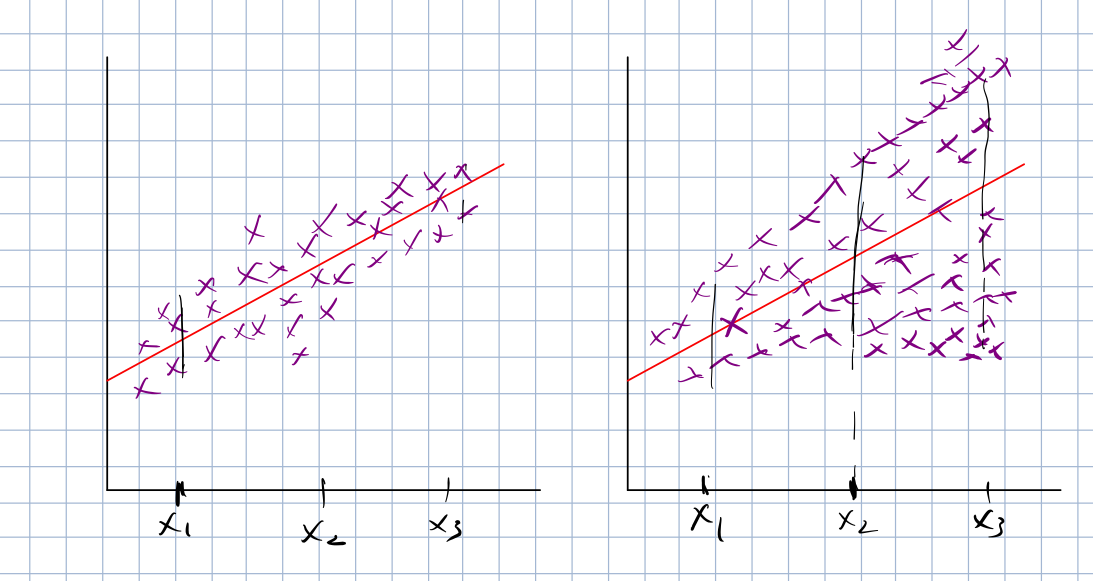
\includegraphics[width=0.55\textwidth]{hetero.png}
\end{figure}
\par\medskip
From the figure, we can see that the variance of the error term changes with $X_i$. In such case, standard errors of our estimators must take this into account. Running two versions of the regression in STATA would help. The homoskedastic version could be obtained by \texttt{regress y x}, while the heteroskedastic version requires \texttt{regress y x, vce(robust)} or \texttt{regress y x, robust}.  Below, I regressed the codes from the previous recitation for comparison. \par\medskip
\begin{figure}[H]
\centering
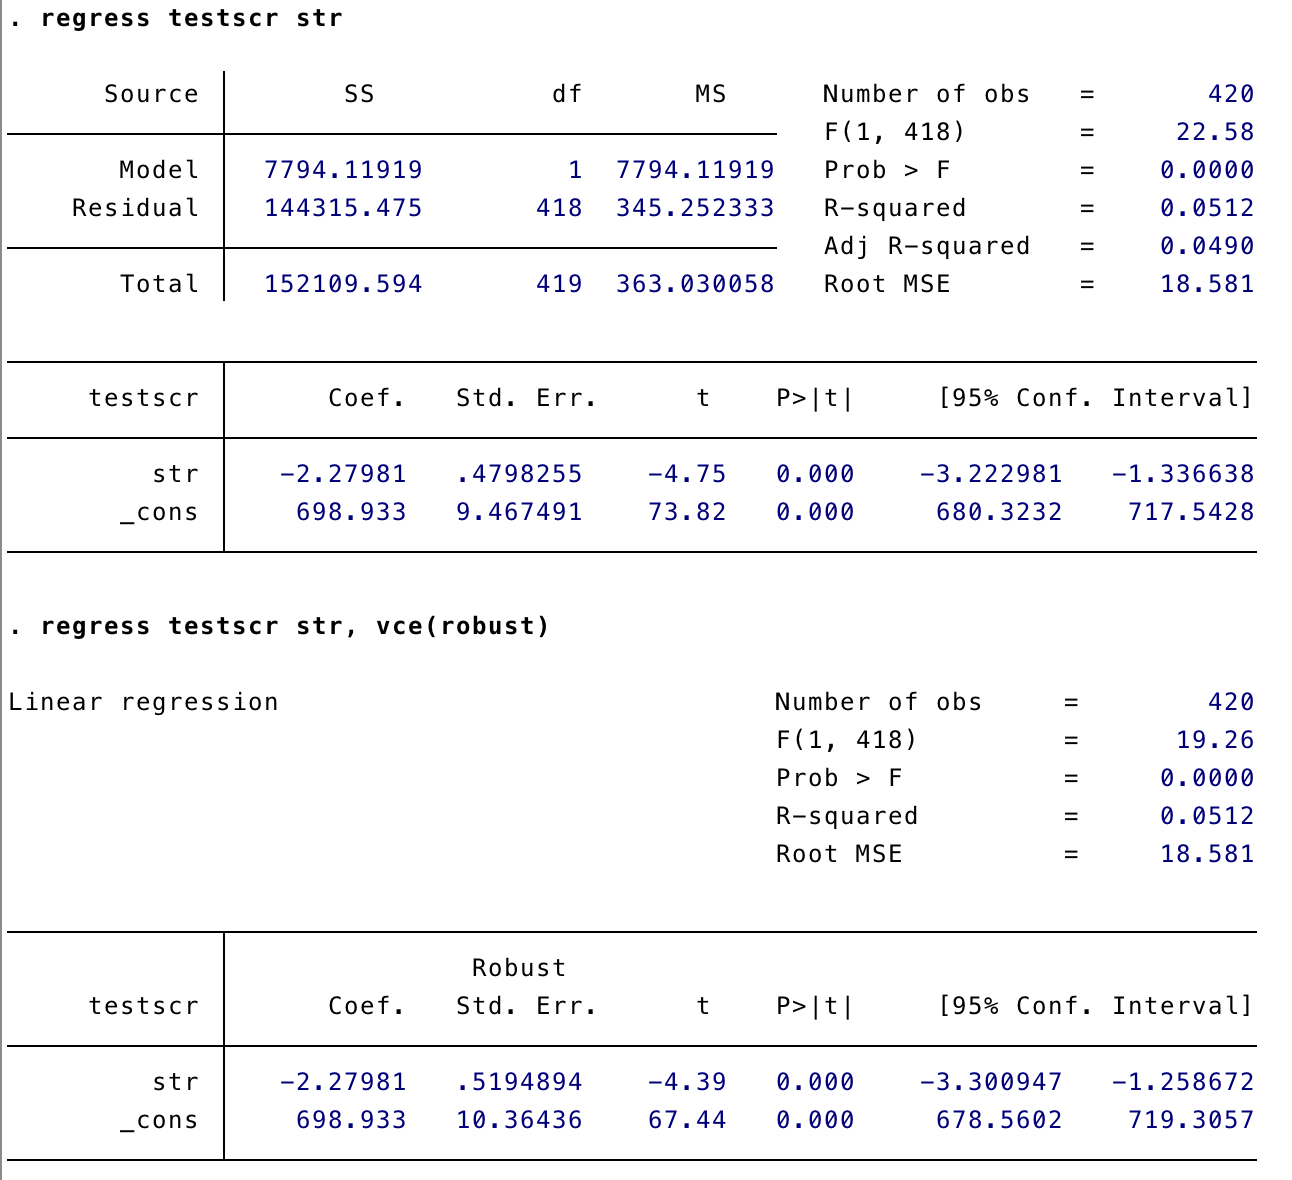
\includegraphics[width=0.7\textwidth]{heterovhomo.png}
\end{figure}
There are two takeaways from the picture
\begin{itemize}
\item \textbf{The variance rises (usually) in the heteroskedastic regression.} In other words, when we keep homoskedasticity assumption in cases where we should not do so, we end up rejecting null hypothesis that should not be rejected.
\item \textbf{The coefficients are unchanged.} When calculating the values for the estimators, we did not rely on the homoskedasticity assumption. Therefore, the coefficients are unaffected. In other words, the estimates are still unbiased.
\end{itemize}

\section{Omitted variable bias}
So far, we have assumed that the number of our independent variable (other than the intercept term) is just one. We now extend our discussion to include more than one independent variable. 
\par\medskip
Before, we regressed whether test score is affected by the size of the classrooms. For every other factor that could affect the test score, we did not include them. However, one might guess that the higher the average income of a county, the higher the test score. Assume that this does affect the test score. Moreover, it is quite likely that richer neighborhoods can afford better school infrastructure and educational quality, leading to smaller size of classrooms. If this is the case, then the model that we have at the moment - without average income of the county - is not capturing the effect of classroom size on test score accurately. \par\medskip 
This is a case of an \textbf{omitted variable bias}. If there is an omitted variable bias, then the estimate we have of the effect of $X_i$ on $Y_i$ is not accurate and thus biased. One formal way to express this issue is as follows: Suppose that the true population regression model and the sample regression model is 
\[
\begin{aligned}
\text{True: }& Y_i = \beta_0 + \beta_1 X_i + \beta_2 Z_i+u_i\\
\text{Mistake: }& Y_i = \beta_0 + \beta_1 X_i + u_i^*\\
\text{Sample: }& Y_i = \hat{\beta}_0 + \hat{\beta}_1 X_i+ \hat{u}_i\\
\end{aligned}
\]
Suppose you run an OLS regression without $Z_i$. As discussed in previous lectures, the OLS estimator for $\beta_1$ can be calculated as $\frac{\sum_{i=1}^n(X_i-\bar{X})(Y_i-\bar{Y})}{\sum_{i=1}^n(X_i-\bar{X})^2}$. However, if you include the $(Y_i-\bar{Y})$ from the true regression model, the OLS estimator now becomes
\[
\begin{aligned}
\frac{\sum_{i=1}^n(X_i-\bar{X})(Y_i-\bar{Y})}{\sum_{i=1}^n(X_i-\bar{X})^2} =& \frac{\sum_{i=1}^n(X_i-\bar{X})(\beta_1(X_i-\bar{X})+\beta_2(Z_i-\bar{Z})+(u_i-\bar{u}))}{\sum_{i=1}^n(X_i-\bar{X})^2}\\
=& \beta_1 + \beta_2\frac{\sum_{i=1}^n(X_i-\bar{X})(Z_i-\bar{Z})}{\sum_{i=1}^n(X_i-\bar{X})^2}+\frac{\sum_{i=1}^n(X_i-\bar{X})(u_i-\bar{u})}{\sum_{i=1}^n(X_i-\bar{X})^2}\\
\end{aligned}
\]
Notice the term $\beta_2\frac{\sum_{i=1}^n(X_i-\bar{X})(Z_i-\bar{Z})}{\sum_{i=1}^n(X_i-\bar{X})^2}$. If $\beta_2 \neq0$ and $\frac{\sum_{i=1}^n(X_i-\bar{X})(Z_i-\bar{Z})}{\sum_{i=1}^n(X_i-\bar{X})^2}\neq 0$, then the mean of $\hat{\beta}_1$ is not guaranteed to be $\beta_1$. This is the reason why omitted variable bias causes inaccurate estimate of $\hat{\beta}_1$. These happen when both of the following cases hold
\begin{itemize}
\item \underline{$Z$ should explain $Y$}: If the slope coefficient of $Z$ is nonzero, then the $Z$ variable is part of the error term if we forget to include them
\item \underline{$Z$ is correlated with $X$}: If $cov(X,Z)\neq0$ and the regression residual $\hat{u}$ is correlated with $Z$, the independent variable is now correlated with $\hat{u}$, which leads to violation of the assumption that independent variable and the residual are not correlated.
\end{itemize} \par\medskip
If both conditions hold, the estimated effect of $X_1$, which is $\hat{\beta}_1$ is not unbiased and is inconsistent. This leads to the result where $E[u^*_i|X_i]=0$ assumption does not hold. There is a formal way to show this with equations.
\par\medskip
With the above formula, we can even determine the direction of the omitted variable bias - whether an estimate is biased downward or upward. The direction of the bias is determined by the sign of the $\beta_2\frac{\sum_{i=1}^n(X_i-\bar{X})(Z_i-\bar{Z})}{\sum_{i=1}^n(X_i-\bar{X})^2}$ term. If this term is positive, then the estimated $\hat{\beta}_1$ becomes larger than the true $\beta_1$. Thus, the estimate is said to be \textbf{overestimated}. If otherwise, $\hat{\beta}_1$ becomes smaller than the true $\beta_1$, making $\hat{\beta}_1$ \textbf{underestimated}.
\par\medskip
In order to address this issue, we can simply include the $Z$ variable if we have the data for it. Another way is to conduct an ideal randomized controlled experiment that randomly assigns \textit{str} to all students. If none of the two are feasible, we should find another variable that can be a proxy to $Z$ - they have to be related to the $X$ variable and is uncorrelated with the errors - which is the Instrumental Variable method. \par\medskip

\section{Multivariate Regression}
\textbf{Multivariate Regression} is simply a regression that involves more than one independent variables. The technicalities involved do not change drastically compared to the univariate regression. However, one should interpret the coefficients cautiously. Suppose that the regression is
\[
Y_i = \beta_0 + \beta_1 X_i + \beta_2 Z_i+u_i
\]
and the variable of interest is $X_i$. To see the impact of $X_i$ and $Y_i$, one needs to take (partial) derivatives on $Y_i$ with respect to $X_i$. This leads to
\[
\beta_1 = \frac{\partial Y_i}{\partial X_i}
\]
In words, $\beta_1$ captures how much $Y_i$ changes with respect to $X_i$ \emph{holding other variables constant} (ceteris paribus). If you do not hold other variables ($Z_i$ in this case) fixed, the change will not exactly be $\beta_1$ (it could be more or less). The statement \emph{holding other variables constant} is crucial in interpreting the $\beta_1$ coefficient.
\par\medskip

%%%%%%%%%%%%%%%%%%







\section{Multivariate Regression: Sampling Statistics}
The estimates for the $\hat{\beta}_j, \ j\in\{0,1,2\}$ can be obtained in a similar way in which we have obtained the OLS estimates for the single variable version. Namely, solve the following minimization problem and get first order conditions with respect to $\beta_0, \beta_1, \beta_2$
\[
\min_{\{\beta_0,\beta_1,\beta_2\}} \sum_{i=1}^n[Y_i-\beta_0 - \beta_1X_{1i}-\beta_2X_{2i}]^2
\]
After some more amount of algebra (than the single variable case), the result we get is the following
\begin{itemize}
\item[$\hat{\beta}_0=$] $\bar{Y}-\hat{\beta}_1\bar{X}_1-\hat{\beta}_2\bar{X}_2$
\item[$\hat{\beta}_1=$] $\frac{\sum_{i=1}^n (X_{1i}-\bar{X}_1)(Y_{i}-\bar{Y})\sum_{i=1}^n(X_{2i}-\bar{X}_2)^2-\sum_{i=1}^n (X_{2i}-\bar{X}_2)(Y_{i}-\bar{Y})\sum_{i=1}^n(X_{1i}-\bar{X}_1)(X_{2i}-\bar{X}_2)}{\sum_{i=1}^n (X_{1i}-\bar{X}_1)^2\sum_{i=1}^n (X_{2i}-\bar{X}_2)^2-[\sum_{i=1}^n (X_{1i}-\bar{X}_1)(X_{2i}-\bar{X}_2)]^2}$
\item[$\hat{\beta}_2=$] $\frac{\sum_{i=1}^n (X_{2i}-\bar{X}_2)(Y_{i}-\bar{Y})\sum_{i=1}^n(X_{1i}-\bar{X}_1)^2-\sum_{i=1}^n (X_{1i}-\bar{X}_1)(Y_{i}-\bar{Y})\sum_{i=1}^n(X_{1i}-\bar{X}_1)(X_{2i}-\bar{X}_2)}{\sum_{i=1}^n (X_{1i}-\bar{X}_1)^2\sum_{i=1}^n (X_{2i}-\bar{X}_2)^2-[\sum_{i=1}^n (X_{1i}-\bar{X}_1)(X_{2i}-\bar{X}_2)]^2}$
\end{itemize} \par\medskip
However, what matters at this point is how we should interpret these coefficients. Suppose that we raise the amount of $X_{1i}$ and leave others unchanged. Then $Y_i$ changes by $\hat{\beta}_1$. Therefore, $\hat{\beta}_1$ measures the change in $Y_i$ due to change in $X_{1i}$ \emph{while leaving other independent variables constant} (ceteris paribus). If other variables are allowed to change, then the change in $Y_i$ due to change in $X_i$ by 1 unit is not guaranteed to be equal to $\hat{\beta}_1$.

\section{Multicollinearity}
When including more independent variables, we are quite likely to end up including independent variables that are highly correlated with each other. \textbf{Multicollinearity} refers to this situation. There are two types of multicollinearities. We say two variables $X_1$ and $X_2$ are \textbf{perfectly multicollinear} if $X_1$ is in an exact linear relationship of some sort with $X_2$. Any multicollinearities that are not in exact linear relationship is referred to as \textbf{imperfect multicollinearity}. \par\medskip

When there is a perfect multicollinearity, we run in to the situation where the denominator and the numerator of the OLS estimates is not defined. These two cases demonstrate possible consequences of multicollinearity
\begin{itemize}
\item \textbf{Assume that $X_2 = cX_1$ for some constant $c$}: Then we have $(X_{2i}-\bar{X}_2)=c(X_{1i}-\bar{X}_1)$. Then $\hat{\beta}_1$ changes to
\scriptsize{\begin{gather*}
\frac{\sum_{i=1}^n (X_{1i}-\bar{X}_1)(Y_{i}-\bar{Y})c^2\sum_{i=1}^n(X_{1i}-\bar{X}_1)^2-c\sum_{i=1}^n (X_{1i}-\bar{X}_1)(Y_{i}-\bar{Y})c\sum_{i=1}^n(X_{1i}-\bar{X}_1)(X_{1i}-\bar{X}_1)}{\sum_{i=1}^n (X_{1i}-\bar{X}_1)^2 c^2\sum_{i=1}^n (X_{1i}-\bar{X}_1)^2-c^2[\sum_{i=1}^n (X_{1i}-\bar{X}_1)(X_{1i}-\bar{X}_1)]^2} \\
=\frac{0}{0} = ???
\end{gather*}}\normalsize
Therefore, $\hat{\beta}_1$ will not be defined (similar for $\hat{\beta}_2$).
\item \textbf{Dummy variable trap}: Say that you have the dummy variable for females and males. Let each of them be $X_{1i}$ and $X_{2i}$ with $X_{2i}=1-X_{1i}$. Then the regression can be written as
\begin{gather*}
Y_i = \beta_0 + \beta_1X_{1i} + \beta_2X_{2i} + u_i \iff Y_i = \beta_0 + \beta_1X_{1i} + \beta_2(1-X_{1i}) + u_i \\
\iff Y_i = \beta_0 + \beta_2 +(\beta_1-\beta_2)X_{1i}+u_i
\end{gather*}
Therefore, by including both $X_{1i}$ and $X_{2i}$ in the same regression, the $X_{2i}$ vanishes from the equation. This is why when you have dummy variables for all categories in the observation, one of them must be left out.
\end{itemize} \par\medskip
The STATA deals with perfect multicollinearity by dropping out some variables that cause perfect multicollinearity.

%%%%%%%%%%%%%%%%%%
\section{Joint testing: Types of Hypothesis Testing}
We have covered hypothesis tests since the beginning of this course. In the regression with single independent variable, we have used $t$-distribution (or if $n$ is sufficiently large, normal distribution) to check whether the following hypothesis hold:
\[
H_0 : \beta_1 = 0 \ \ H_1 : \beta_1 \neq 0
\]
and the test statistic was (assuming homoskedasticity)
\[
t=\frac{\hat{\beta}_1-0}{s.e(\hat{\beta})}\sim t_{n-2} \ \ (\sim N(0,1) \ \text{in large samples})
\]
where $s.e(\hat{\beta}_1)=\sqrt{\frac{1}{n}\frac{\frac{1}{n-2}\sum_{i=1}^n(X_i-\bar{X})\hat{u}_i}{(\frac{1}{n}\sum_{i=1}^n (X_i-\bar{X})^2)^2}}$. So it may seem plausible to think that to test the hypothesis on a setting where we have multiple independent variables, we just need to run this many times. However, this is not exactly the case. the following example demonstrates why. \\ \par

\begin{mdframed}[backgroundcolor=blue!5] 
\textbf{Why do multiple testing using $t$-statistics have problems?} \medskip \\ 
Consider the case where there is you are testing on multiple independent variables. Suppose that you are running a two-sided test with 5 independent variables and significance level $\alpha = 5\%$ under the null hypothesis
\[
H_0: \beta_1=...\beta_5=0
\]
You reject the null hypothesis when $|t_i|\geq 1.96 \ i\in\{1,2,3,4,5\}$ Note that for each $i$, the probability of $|t_i|\geq 1.96$ is 0.05. Now assume that each test statics are independent. Then the probability of incorrectly rejecting the null hypothesis using this approach is
\[
\begin{aligned}
\Pr(|t_1|>1.96 \cup...\cup |t_5|>1.96) & =1-\Pr(|t_1|\leq1.96\cap .. \cap|t_1|\leq1.96)\\
(\because\text{Independence of $t_i$'s}) \ \ &=1-\Pr(|t_1|\leq1.96)\times ..\times\Pr(|t_5|\leq1.96) \\
 & = 1-(0.95)^5 \\
 &= 0.2262
\end{aligned}
\]
This means that the rejection rate under the null is not 5\% but 22\% percent. Therefore, we end up rejecting the null hypothesis more than we have to. (Formally, we say that the probability of type 1 error rises sharply.) 
\end{mdframed} \par\medskip
Because of this fact, we require another approach when testing multiple hypotheses at the same time. This is where \textbf{$F$-test} comes in. This is a test where all parts of the joint hypothesis can be tested at once. It also has mechanism for correcting the correlation between the $t$-test statistics. It ultimately allows us to correctly set the significance level even for the multiple testing case. \par\medskip
The usual joint hypothesis test for the regression with $k$ variables (not including the constant term) is
\[
H_0: \beta_1 = ... =\beta_k=0, \ H_1:\lnot H_0
\]
where $H_1$ refers to the case where there is a nonzero element in any one of $\beta_1$ to $\beta_k$. The $\lnot$ symbol refers to ``not". Note that the default F-test null hypothesis for STATA is $H_0:\beta_1 = ... =\beta_k=0$ and $H_1: \lnot H_0$.\par\medskip
We can actually go farther. Suppose that instead of $\beta_1$ and $\beta_2$ being zero, we are just interested in whether they are equal. The $F$-test can also be used for testing this hypothesis. The setup of the hypothesis would be
\[
H_0: \beta_1 = \beta_2 \ H_1: \beta_1 \neq \beta_2
\]
I will discuss how to implement such hypothesis test on STATA in the next section. \par\medskip
\noindent
\textit{For curious minds: } Note that the square of the $t$ distribution with the degree of freedom $n$ is equivalent to the $F$ distribution with $1$ degree of freedom in the numerator and $n$ in the denominator. For more information, please refer the link I attach in the footnotes\footnote{\url{http://homepage.stat.uiowa.edu/~rdecook/stat3200/notes/t_and_F_4pp.pdf}}
\section{Interpreting the Results}
Below are the results of a regression on multiple variables. I am using the data from Professor Almond's paper on cost of low birthweight\footnote{Almond, Douglas, Kenneth Chay, David Lee (2005) ``The Costs of Low Birthweight", \textit{Quarterly Journal of Economics} 120(3):1031-1083}. I regress \textit{birthweight} on \textit{smoker, alcohol, Nprevist} (number of prenatal visits to doctor).
\begin{figure}[H]
\begin{center}
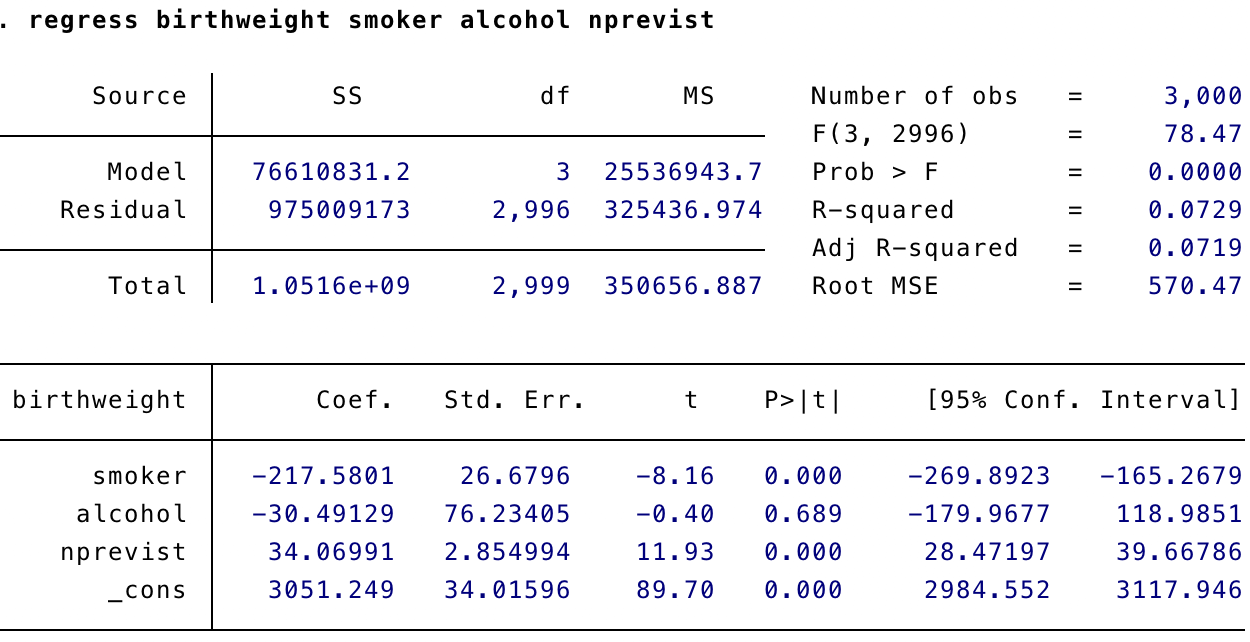
\includegraphics[width=0.7\textwidth]{regoutput.png}
\end{center}
\end{figure}\par\medskip
You can see that running multivariate regression is similar in terms of the techniques involved. Additional complication rises from interpreting the goodness of fit. In addition to $R^2$, we now get the \textbf{adjusted $R^2$}, which is defined as
\[
\bar{R}^2 = 1-\frac{n-1}{n-k-1}\frac{\text{Residual Sum of Squares}}{\text{Total Sum of Squares}}
\]
Since we are assuming that $k\geq 1$, adjusted $R^2$ is smaller than the $R^2$. As we include more variables, the $\frac{n-1}{n-k-1}$ increases, leading to further decrease in adjusted $R^2$. However, if the new variables are very relevent, $\frac{\text{Residual Sum of Squares}}{\text{Total Sum of Squares}}$ decreases. This reduces the gap between $R^2$ and the adjusted $R^2$. If the adjusted $R^2$ do not decrease drastically, it is a sign that we are adding a relevant variable. \par\medskip
One way to conduct various hypothesis testing is to utilize the \texttt{test} command. I include two pictures, one with $H_0: \beta_{\text{smoker}}=\beta_{\text{alcohol}}=\beta_{\text{nprevist}}=0$ on the left and the other with $H_0:\beta_{alcohol}+\beta_{nprevist}=0$ on the right.
\begin{figure}[H]
\begin{center}
        \begin{subfigure}[b]{0.45\textwidth}
	\centering
                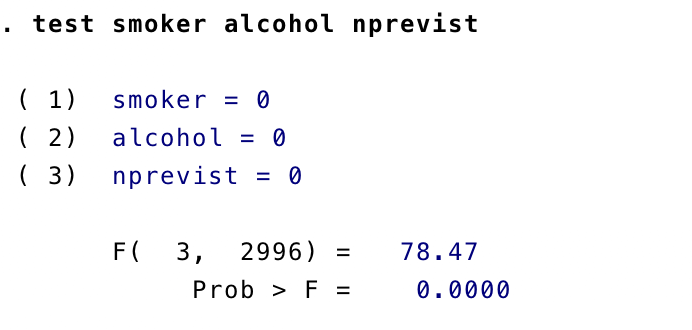
\includegraphics[width=\linewidth]{test}
        \end{subfigure}
        \begin{subfigure}[b]{0.45\textwidth}
	\centering
                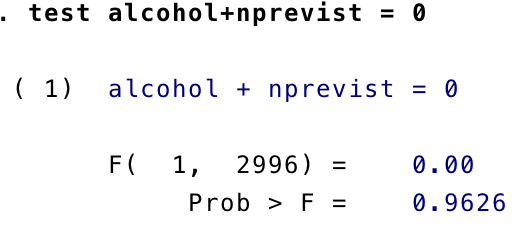
\includegraphics[width=\linewidth]{test1}
        \end{subfigure}
\end{center}
\end{figure}



%%%%%%%%%%%%%%%%%%
\section{F-tests}
You should know after the problem sets that you use $F$-tests to assess the results of a joint hypothesis. The \textbf{$F$-statistics} are calculated in two ways. One uses $t$-statistics from individual hypotheses. This is calculated as
\[
\frac{1}{2}\left(\frac{t_1^2+t_2^2-2\hat{\rho}_{t_1,t_2}t_1t_2}{1-\hat{\rho}^2_{t_1,t_2}}\right)
\]\par\medskip
Another one, which is useful for calculating $H_0: \beta_1 = ... =\beta_q=0$ hypothesis ($q$ is the number of hypotheses being tested on) uses $R^2$ from the 'unrestricted' and 'restricted' regressions. Assume that there are total of $k$ independent variables, where $k\geq q$ and the null hypothesis is as stated above. The restricted regressions and unrestricted regressions are defined as
\[\begin{aligned}
\text{Restricted: } & Y_i =\beta_0+ 0X_{1,i} + ...+ 0X_{q,i}+ \beta_{q+1}X_{q+1,i}+...+\beta_kX_{k,i} + u_i\\
\text{Unrestricted: } & Y_i = \beta_0+\beta_1X_{1,i} + ... +\beta_qX_{q,i}+ \beta_{q+1}X_{q+1,i}+...+\beta_kX_{k,i} + u_i\\
\end{aligned}\] \par\medskip
You can now notice that restricted regression assumes that $H_0$ is true and then only optimizes with respect to $\beta_{q+1},...,\beta_{k}$. Unrestricted regression does not assume that $H_0$ is true and optimizes with respect to all slope coefficients. The second formula for $F$-statistic uses $R^2$ from these two regressions. Intuitively, the unrestricted regression allows for the role of $X_1,..,X_q$ whereas their role in restricted regression is limited. This is why $R^2$ in unrestricted regression is higher than restricted regression. Given this, $F$-statistic is
\[
\frac{(R^2_{\text{Unrestricted}}-R^2_{\text{Restricted}})/q}{(1-R^2_{\text{Unrestricted}})/(n-k-1)}
\]
where $k$ is total number of independent variables (not counting intercept) and $q$ is the number of restrictions. \par\medskip
There is another way to express this. Note that $R^2_{\text{Restricted}} = 1-\frac{RSS_{\text{Restricted}}}{TSS}$. $R^2_{\text{Unrestricted}}$ is defined similarly. By using this and with little algebra, we can derive this formula, which is mentioned in most econometrics textbooks.
\[
\frac{(RSS_{\text{Restricted}}-RSS_{\text{Unrestricted}})/q}{(RSS_{\text{Unrestricted}})/(n-k-1)}
\] \par\medskip


\section{Control variables and conditional mean independence}
Assume that we have a following setup:
\[
\begin{aligned}
\text{True: }& Y_i = \beta_0 + \beta_1 X_i + \beta_2 Z_i+u_i\\
\text{Mistake: }& Y_i = \beta_0 + \beta_1 X_i + u_i^*\\
\text{Sample: }& Y_i = \hat{\beta}_0 + \hat{\beta}_1 X_i+ \hat{u}_i\\
\end{aligned}
\]
If we end up with an omitted variable bias by not including $Z_i$, Then, we have a problem. We can see this from
\[
\begin{aligned}
E[u_i^*|X_i]&=E[\beta_2Z_i+u_i|X_i]\\
&=\beta_2Z_i+E[u_i|X_i] \neq 0
\end{aligned}
\]
So Assumption 2 from the classical linear regression model (refer to Recitation 3), fails and $\hat{\beta}_1$ without inclusion of $Z_i$ is biased. To address this, we ideally add this variable into the regression. That may not always be possible. In that case, we can find $W_i$ variable that is correlated with $Z_i$ to some extent and include that in the regression. By doing so, we achieve three things
\begin{itemize}
\item The $u_i$ term is no longer correlated with $X_i$ ($cov(X_i, u_i)=0$)
\item For given value of $W_i$, then the variable of interest $X_i$ is no longer correlated with the omitted determinant of $Y_i$
\item For given $W_i$, $X_i$ acts as if they are randomly assigned
\end{itemize}
Variable $W_i$ that achieves this is called an \textbf{effective control variable}. In this particular case, we say that the \textbf{conditional mean independence} hold, in the sense that as long as we control for $W_i$, $u_i$ is independent of $X_i$ - making our coefficient of interest unbiased. 
\[
E[u_i|X_i,W_i]= E[u_i|W_i]
\]
Note that $W_i$ itself does not need to have causal relationship with $Y_i$
%%%%%%%%%%%%%%%%%%
\section{Nonlinear regressors: Motivation}
Not everything in real life is correlated in a linear fashion. For instance, production function are not usually linear with respect to its inputs (Cobb-douglas production function), Wage rises, but the rate at which it rises falls over time (Mincer equation, from Mincer (1974)\footnote{\scriptsize{Mincer, Jacob (1974) "Schooling, Experience, and Earnings", New York, National Bureau of Economic Research}}), and the effect of classroom size can differ depending on how many students are in the class to begin with(Lazear(2001)\footnote{\scriptsize{Lazear, Edward (2001) "Educational Production", \textit{Quarterly Journal of Economics}, 116(3): 777-803}}). \par\medskip
For correlations like this, resorting to linear regressors would not allow the regression model to have the best fit. This is where the nonlinear regressors come in. Regressions with nonlinear regressors allow us to graph relationship between our $Y$ variable and our $X$ variable that is not necessarily linear. When incorporating such regressors, the interpretation of each coefficient becomes trickier. In the next few subsections, I will walk through implementing and interpreting coefficients for regressors that are not linear. \par\medskip
\section{Quadratic terms}
Recall from the regression with single independent variable $Y= \beta_0 + \beta_1X_1+u$, $\beta_1$ coefficient means the marginal effect of $X_1$ on $Y$. Mathematically, there are two ways to show this. (For now, all usual assumptions hold)
\begin{itemize}
\item \textbf{Derivatives}: Take derivatives on $Y$ with respect to $X_1$, this gets us
\[
\frac{\partial Y}{\partial X_1} = \frac{\partial}{\partial X_1}[ \beta_0 + \beta_1X_1+u ] = \beta_1
\]
Given that the idea of derivatives captures how much our $Y$ variable changes with unit change in $X_1$, $\beta_1$ represents how much $Y$ responds to a one unit change in $X_1$
\item\textbf{Taking Differences}: Suppose that you raise the amount of $X_1$ by $\Delta x$. Now the change in the  amount of $Y$, denoted as $\Delta y$, as a result of this change is
\[
\beta_0 + \beta_1(X_1+\Delta x)+u = Y+\Delta y
\] 
By subtracting $Y= \beta_0 + \beta_1X_1+u$, I get
\[
\Delta y = \beta_1 \Delta x \implies \frac{\Delta y}{\Delta x} = \beta_1
\]
\end{itemize} \par\medskip
In this example, the marginal effect of $X$ on $Y$ is constant - it does not depend on $X$! However, there are many relationships that cannot be explained this way. For instance, it is most likely the case that the wage rises with age. However, they are not likely to be in a linear relationship. As one gets older, the rate at which wage increases with age decreases. This is where \textbf{polynomial regressors} can improve the fitting of the regression model. Let wage be $W$ and age be $X$. I now regress the following model.
\[
W = \beta_0 + \beta_1 X+ \beta_2 X^2+u
\]
Then, the marginal impact of age on wage can be captured by
\[
\frac{\partial W}{\partial X} = \beta_1 + 2\beta_2 X
\]\par\medskip
Note now that unlike before, there is a term that depends on $X$. This implies that the marginal effect of age on wage now is different depending on what $X$ variables we use (or age). When $\beta_2$ is positive (negative), then marginal impact of age on wage is higher (lower) for older people. Simply put, age rises at faster (slower) rate for older people. \par\medskip





%%%%%%%%%%%%%%%%%%
\chapter{Panel Regression}
\section{Motivation for Using Panel Data}
We now get to analyze a different type of dataset. We are moving into the \textbf{panel data}, where we observe multiple individuals for multiple periods of time. In terms of notation, we write
\[
Y_{it} = \beta_0 + \beta_1X_{1,it}+ ... +\beta_kX_{k,it}+u_{it}
\]
where $i=1,2,...,N$ indicates individuals and $t=1,2,...,T$ indicates time periods. For some panel datasets, there are $T$ datasets for each of the $N$ individuals included in the data. This type of panel data is said to be a \textbf{balanced panel data}. However, most panel data available to public has cases where there are $t\leq T$ datapoints for some of the $N$ individuals. This type of dataset is an \textbf{unbalanced panel data}. \par\medskip
There are many reasons for using a panel data. One is simply that using a panel data allows us to use more datasets. As we have learned from the previous lectures, our estimates get easier and more accurate as we have more data. However, a crucial advantage of using a panel dataset comes from the fact that it can allow us to control for a particular type of omitted variable bias. Specifically, it can allow us to control for \textbf{unobserved heterogeneity} that are either 1) different accross $N$ entities but always remain same for $T$ periods in a given state or 2) different accross $T$ times periods but remains the same for all $N$ entities in a particular time period or 3) both of 1) and 2). The first of this is called a \textbf{cross section fixed effect}. The second one is \textbf{time fixed effects}. Case 3) is what we call \textbf{two-way fixed effects}.\par\medskip
\begin{mdframed}[backgroundcolor =blue!10]
\textit{For curious minds}: Can the unobservable heterogeneity be unrelated to the independent variables? In theory, yes. This type of unobserved heterogeneity is commonly referred to as \textbf{random effects}. In reality, not many data satisfy this. So we will delay the discussion of this topic to an advanced course 
\end{mdframed} \par\medskip
To see why that is the case, suppose that $T=2$ and we are interested in the relationship between vehicle related fatality rate (deaths per 10,000 people) and the beer tax. Suppose that we get these result for the two years
\[
\begin{aligned}
\hat{Y}_{i1} &=2.01 &+ 0.15X_{i1}\\
                    &(0.15)&(0.20) \\
\hat{Y}_{i2} &=1.86 &+ 0.44X_{i2}\\
                    &(0.11)&(0.20) \\                    
\end{aligned}
\]
In the first year, the coefficient on $X_i$ is not significant at all, whereas the same coefficient for year 2 is very significant. In such case, one might suspect that there is an omitted variable bias that affects these coefficients. For instance, if $i$ denotes states, one might guess that some type of omitted variable that are specific to the states could be affecting these results - like strictness of DUI laws in some state $i$. If it is the case that the strictness of DUI laws did not change for the two time periods, then these effects qualify as a state fixed effect (replace cross section with state). \par\medskip 
To see how such omitted variable bias can be controlled for, let $Z_i$ denote the strictness of state laws on DUI. This is not exactly measurable. However, if there is no significant change in state law for the two periods, $Z_i$ can be considered unchanging. Now write
\[
\begin{aligned}
Y_{i1}& = \beta_0 + \beta_1X_{i1}+\beta_2 Z_{i}+u_{i1} \\                
Y_{i2}& = \beta_0 + \beta_1X_{i2}+\beta_2 Z_{i}+u_{i2} \\                
\end{aligned}
\]
Subtract the second equation from the first to get
\[
(Y_{i2}-Y_{i1}) = \beta_1(X_{i2}-X_{i1}) +\beta_2(Z_{i}-Z_{i}) + u_{i2}-u_{i1}
\]
With $Z_i$ being the same for all periods, the above equation is reduced to
\[
(Y_{i2}-Y_{i1}) = \beta_1(X_{i2}-X_{i1}) +(u_{i2}-u_{i1})
\]
The $Z_i$ variable has no role in this equation. Effectively, we did control for state fixed effect that are constant across time. If we estimate this particular $\beta_1$, we can obtain much more accurate estimates of the effect of bear tax on fatality rate. The $\beta_1$ in this case can be interpreted as how much the change in ($X_{i2}-X_{i1}$) changes ($Y_{i2}-Y_{i1}$). \par\medskip
Let's use a numerical example, Suppose that beer tax is \$10 in year 1, so $X_{i1}=10$. Suppose that state $i$ raises its bear tax by $1$ dollars, therefore $X_{i2}-X_{i1}=1$. If $\beta_1$ is estimated as  $-1.1$, then we can write the predicted change in $Y$ (which would be a predicted change in death per 10,000 people) as
\[
\widehat{Y_{i2}-Y_{i1}} = -1.1(X_{i2}-X_{i1})
\]
If you put  $X_{i2}-X_{i1}=1$, Then $\widehat{Y_{i2}-Y_{i1}} = -1.1$, or that fatality per 10,000 reduces by 1.1. Also notice that this is starkly different result compared to the estimates we got when we regressed year by year (coefficient in front of $X$ was positive, as opposed to a negative coefficient for change in $X$ we used for the second approach). \par\medskip
\section{Methodology}
We are going to limit our discussion to a cross-sectional fixed effects, as all logic would hold by changing cross sectional index $i$ to time index $t$. For each of these fixed effects, there are two ways of estimating the data when $T\geq 3$. One of them is to include $N-1$ individual dummy variables (or $T-1$ time period dummy variables), sometimes referred to as \textbf{least square dummy variable method}. The other is to subtract from the original equation the ``demeaned" equation, which is referred to as \textbf{within estimation}. \par\medskip
For both approaches, the following framework will work. Assume that the true relation between $Y$ and $X$ variable is 
\[
Y_{it}=\beta_0 + \beta_1X_{it}+\beta_2 Z_{i}+u_{it} \tag{1}
\]
where $Z_i$ is the cross section fixed effect. For $i=1,...,N$, the value of $\beta_2 Z_i$ is different. If we were to express this equation on an $(X,Y)$-plane, we would end up with a different intercept for each $i$. So for simplification, define $\alpha_i = \beta_0 + \beta_1Z_i$. Then the above equation can be written as
\[
Y_{it}=\beta_1X_{it}+\alpha_{i}+u_{it} \tag{2}
\]
in equation (2), the $\alpha_i$ term can be thought of as an effect of being an entity $i$. Since this is correlated with $X_{it}$, we deal with this in two ways
\subsection{Least Square Dummy Variable Method}
For this, we are going to make changes to equation (1). Define a new variable $D_{ki}$ as follows
\[
D_{ki} = \begin{cases} 1 & \text{If $i=k$} \\
                                     0 & \text{Otherwise } \end{cases} , \ k\in\{1,2,...,N\}
\] 
This variable takes 1 if $i$ is the $k$th entity. We are defining this for all $N$ entities. Since we are going to include $\beta_0$, a common intercept, in our regression we need to remove one of the $N$ $D_{ki}$ variables out to avoid dummy variable trap. Let's remove $D_{1i}$ from the equation and include all others, then equation (1) becomes
\[
Y_{it} = \beta_0 +\beta_1X_{it}+\delta_2D_{2i} + ... + \delta_ND_{Ni}+u_{it} \ \tag{LSDV}
\]
To see what this equation gives, we analyze what the intercept will be for each of the $N$ entities. This can be written out as
\[
\begin{aligned}
i=1 \implies & (1): \beta_0 + \beta_2Z_1 &(2): \alpha_1 \ & (3): \beta_0\\ 
i=2 \implies & (1): \beta_0 + \beta_2Z_2 &(2): \alpha_2 \ & (3): \beta_0+\delta_2\\ 
...&...&...&...\\
i=N \implies & (1): \beta_0 + \beta_2Z_N &(2): \alpha_N \ & (3): \beta_0+\delta_N\\ 
\end{aligned}
\]
In all of these cases, slope coefficient in front of $X_{it}$ remains the same. In addition, we control for unobserved cross section fixed effect by allowing the intercept to differ by each $i$. \par\medskip
One clear disadvantage of this method is the computational burden when $N$ or $T$ is large. If $N$ is extremely large, this cannot be solved on pen(cil) and paper. It may even take computer quite a lot of time to process the results. The computational burden cam be eased with the following method. \par\medskip
\subsection{Within Transformation Method}
Go back to equation (2). Since we are concerned about cross section fixed effects, we define a new term, $\bar{X}_i, \bar{Y}_i$ as sample mean of $X_{it}, Y_{it}$ for some given $i$ over all possible $t$'s. This can be calculated as
\[
\bar{X}_i = \frac{1}{T}\sum_{t=1}^TX_{it}
\]
Consequently, $\bar{Y}_i$ can be written as
\[
\bar{Y}_i = \frac{1}{T}\sum_{t=1}^TY_{it}=\frac{1}{T}\sum_{t=1}^T\left(\beta_1 X_{it} +\alpha_i +u_{it}\right)=\beta_1 \bar{X}_i +\alpha_i + \bar{u}_{i}
\]
where $\bar{u}_i$ is defined in a similar manner to $\bar{X}_i, \bar{Y}_i$. Then, we subtract $Y_{it}$ by $\bar{Y}_i$ to get
\[
\begin{aligned}
Y_{it}-\bar{Y}_i &= \beta_1(X_{it}-\bar{X}_i) + (u_{it}-\bar{u}_i)\\
\implies \tilde{Y}_{it}&= \beta_1 \tilde{X}_{it}+\tilde{u}_{it}\\
\end{aligned}
\]
where $\tilde{X}_{it}= (X_{it}-\bar{X}_i)$. This controls the fixed effect term by effectively getting rid of them through this transformation process (also known as within transformation). To get the $\beta_1$ estimate, we solve the minimization problem similar to what we have went through in finding the original OLS estimator. This gets us
\[
\hat{\beta}_1= \frac{\sum_{i=1}^n \sum_{t=1}^T \tilde{X}_{it}\tilde{Y}_{it}}{\sum_{i=1}^n \sum_{t=1}^T \tilde{X}_{it}^2}
\]
\begin{mdframed}[backgroundcolor =blue!10]
\textbf{Within estimator}: Again, the minimization problem is to find the $\hat{\beta}_1$ that minimizes the sum of the squared residual terms. This is written as
\[
\min_{\hat{\beta}_1} \sum_{i=1}^N \sum_{t=1}^T (\tilde{Y}_{it}-\hat{\beta}_1 \tilde{X}_{it})^2
\]
Differentiate this term with respect to $\hat{\beta}_1$ to get this first order condition
\[
-2\sum_{i=1}^N \sum_{t=1}^T (\tilde{Y}_{it}-\hat{\beta}_1 \tilde{X}_{it})\tilde{X}_{it}=0
\]
Solving this, we can get $\hat{\beta}_1= \frac{\sum_{i=1}^n \sum_{t=1}^T \tilde{X}_{it}\tilde{Y}_{it}}{\sum_{i=1}^n \sum_{t=1}^T \tilde{X}_{it}^2}$. 
\end{mdframed} \par\medskip
For time fixed effects, all of our logic remains similar. The exception is that we now need to use $\bar{Y}_t$, defined as
\[
\bar{Y}_t = \frac{1}{N}\sum_{i=1}^N(Y_{it}) = \beta_1 \bar{X}_t +\alpha_t +\bar{u}_t
\]
\subsection{Time and Entity Fixed Effects}
This is sometimes called a \textbf{two-way fixed effect models}. This is written by
\[
Y_{it}=\beta_1 X_{it} + \alpha_i +\lambda_t + u_{it}
\]
As with the previous fixed effect models, there are two ways to deal with this
\begin{itemize}
\item \textbf{Least square dummy variable}: Now, we include $N-1$ and $T-1$ binary independent variables, along with a common intercept $\beta_0$ to get
\[
Y_{it} = \beta_0 +\beta_1X_{it}+\gamma_2T_{2t}+...+\gamma_TT_{Tt}+\delta_2D_{2i} + ... + \delta_ND_{Ni}+u_{it} 
\]
\item \textbf{Within estimator}: This is a bit complicated, but possible. When both time and entity fixed effects are present, the way of demeaning the data is different. We first demand by time and entity, and then add back the overall sample mean back. In other words, the demeaning process is 
\[
Y_{it}-\bar{Y}_i -\bar{Y}_t +\bar{Y}
\]
where $\bar{Y} = \frac{1}{NT}\sum_{i=1}^N \sum_{t=1}^TY_{it}$ and 
\begin{itemize}
\item $\bar{Y}_i = \beta_1 \bar{X}_i +\alpha_i +\frac{1}{T}\sum_{t=1}^T\lambda_t+\bar{u}_i$
\item $\bar{Y}_t = \beta_1 \bar{X}_t +\frac{1}{N}\sum_{i=1}^N\alpha_i +\lambda_t+\bar{u}_t$
\item $\bar{Y}  =\beta_1\bar{X}+\frac{1}{N}\sum_{i=1}^N\alpha_i+\frac{1}{T}\sum_{t=1}^T\lambda_t+\bar{u}$
\end{itemize}
Then, we get
\[
(Y_{it}-\bar{Y}_i -\bar{Y}_t +\bar{Y}) = \beta_1(X_{it}-\bar{X}_i -\bar{X}_t +\bar{X}) + (u_{it}-\bar{u}_i -\bar{u}_t +\bar{u})
\]
We conduct the OLS estimation here to get the estimate for $\beta_1$. 
\end{itemize}
\subsection{Least Square Assumption for Panel Data}
The following assumptions are extensions from what we had in the cross sectional data. However, there are some key differences that are observed in the panel data setting. The four main assumptions are
\begin{itemize}
\item [\textbf{P1}]: $E[u_{it}|X_{i1},..,X_{iT},\alpha_i]=0$. It means that the conditional mean of the $u_{it}$ term does not depend on any of the $X_{it}$ values for entity $i$, whether in the future or in the past. This rules out omitted variable bias. Some books refer to this as strict exogeneity. 
\item [\textbf{P2}]: $(X_{i1},..,X_{iT},u_{i1},...u_{iT})$ is IID across $i=1,..,n$. In other words, variables for one entity are distributed identically to but independent of other entities. However, \textbf{this does not rule out the correlation between $u_{it},u_{ij}$ within entity $i$ for different $j$ and $t$}. Therefore, within an entity, there could be an autocorrelation (or serial correlation).  
\item [\textbf{P3}]: $(X_{it},u_{it})$ have nonzero finite fourth moments. In other words, outliers are very unlikely. We need this condition to derive the asymptotic distribution of the estimators in the panel regression. (Not a scope of this class)
\item [\textbf{P4}]: There is no perfect multicollinearity
\end{itemize}
Because of \textbf{P2}, the standard errors should be calculated while taking into account the possibility of autocorrelation within an entity. This is where \textbf{clustered standard error} comes in. This type of standard errors allow for heteroskedasticity and autocorrelation within an entity. However, it assumes that regression errors are independent across different entities. In practice, clustered standard errors are larger than regular standard errors (but not always). As in the case of heteroskedasticity, we should care about clustering as using ``wrong" standard errors would lead us to making a wrong judgement about the hypothesis we set on some variables. \par\medskip






%%%%%%%%%%%%%%%%%%
\chapter{Binary Dependent Variables}
\section{Linear Probability Models}
We now turn to the case where the dependent variable $y$ takes either 0 or 1. This type of regression can be used to study how independent variable(s) $X_i$ is(are) correlated to yes/no questions in the survey. As always, assume a following regression equation
\[
Y_i = \beta_0 + \beta_1 X_i +u_i
\]
where $Y_i$ is a binary variable.  Unlike previous regressions, the complication arises when we attempt to interpret the equation. Especially, what does $\beta_1$ now mean? To study this question, we first look into the expected value of $Y_i$ conditional on $X_i,\ E[Y_i|X_i]$. The conditional mean of $Y_i$ is, by definition
\[
E[Y_i|X_i] = 0\times\Pr(Y_i=0|X_i)+1\times\Pr(Y_i=1|X_i)
\]
In the context of this regression equation, we can obtain the conditional mean of $Y_i$ as follows
\[
\begin{aligned}
E[Y_i|X_i]&=E[\beta_0+\beta_1X_i+u_i|X_i]\\
&=\beta_0 + \beta_1X_i + E[u_i|X_i]\\
(\because  E[u_i|X_i]=0)&=\beta_0 + \beta_1X_i 
\end{aligned}
\]
Therefore, we just established that $E[Y_i|X_i]$ in this context is the probability of $Y_i=1$ given $X_i$. \par\medskip
Now we move back to $\beta_1$, notice that $\beta_1 =\frac{\Delta Y_i}{\Delta X_i}$ and $\Delta Y_i = \text{Change in }\Pr(Y_i=1|X_i)$ with respect to change in $X_i$ , or
\[
\Delta Y_i = \Pr(Y_i=1|X_i=x+\Delta X_i)-\Pr(Y_i=1|X_i=x)
\]
and when we calculate $\Pr(Y_i=1|X_i=x+\Delta X_i)-\Pr(Y_i=1|X_i=x)=E[Y_i|X_i=x+\Delta X_i]-E[Y_i|X_i=x]$, we get
\[
\beta_0+\beta_1(x+\Delta X_i)-\beta_0+\beta_1(x) =\beta_1 \Delta X_i
\]
So we get $\Delta Y_i = \beta_1\Delta X_i\iff\beta_1 =\frac{\Delta Y_i}{\Delta X_i}$. Therefore, $\beta_1$ now measures how much the predicted probability of $Y_i=1$ changes with respect to $X_i$ \par\medskip
The \textbf{linear probability model} is the estimation in which you run an OLS on the type of regression equation where $Y_i$ is a binary dependent variable. The advantage is that it is simple - there is no difference in terms of methods between this and the OLS methods we have learned so far. However, there are some critical disadvantages to this model. One is that by setting the regression model as above, we are assuming that the change of predicted probability of $Y_i=1$ is constant for all values of $X_i$. But more critically, it is possible that because of the way functional form is specified, the predicted probability $\hat{y}$ may be greater than 1 or strictly less than 0. Given that probability is defined to be in between 0 and 1, this could be a preposterous result. In addition, the distribution of the error term is no longer normal distribution. This could affect the asymptotic (large sample) properties of the OLS estimators. \par\medskip
\section{Logit and Probit Regressions}
Since linear probability models can exceed 1 or fall below 0, we now use a class of \textbf{sigmoid estimators}. These estimators are bounded between 0 and 1. Therefore, using these estimators will prevent the predicted probability of $Y_i=1$ falling out of $[0,1]$ range. \par\medskip
One of such estimator is \textbf{logit regression}. For notational convenience, I write $Z_i=\beta_0+\beta_1X_i$. Logit regression assumes that the cumulative probability of $Z_i$, which is $\Pr(Y_i=1|X_i)$  is distributed as
\[
\Pr(Y_i=1|X_i)=F(Z_i)=\frac{1}{1+e^{-Z_i}}
\]
In this setup, when $Z_i\to\infty, e^{-Z_i}\to0$ Therefore, $F(Z_i)\to1$. Likewise, taking $Z_i\to-\infty$ results in $F(Z_i)\to0$. \par\medskip
To see the role of the independent variable $X_i$, we should note that changes in $X_i$ leads to changes in $Z_i$, since $Z_i = \beta_0+\beta_1X_i$. The change in $Z_i$ should also impact $F(Z_i)$. Borrowing the logic from the chain rule, we get
\[
\frac{\partial F}{\partial X_i} = \frac{\partial F}{\partial Z_i}\frac{\partial Z_i}{\partial X_i}  
\]
where $\frac{\partial Z_i}{\partial X_i}  =\beta_1$. This says that $\beta_1$ alone does not explain how changes in $X_i$ alters probability of $Y_i=1$ given $X_i$.  Therefore, the coefficient value of $\beta_1$ does not mean that much in logit regression (similar for probit regressions). However, Note that $ \frac{\partial F}{\partial Z_i}$ is calculated as
\[
 \frac{\partial F}{\partial Z_i}=\frac{e^{-\beta_0 -\beta_1X_i}}{(1+e^{-\beta_0 -\beta_1X_i})^2}
\]
Therefore the sign of $\beta_1$ still matters. In fact, the interpretation of logit coefficients (and probit) regression matters up to the sign of the coefficients in general. \par\medskip
\textbf{Probit regression} is largely similar with the logit regression, except now that the cumulative probabiltiy of $Z_i$ is assumed to be a standard normal function. Specifically, 
\[
F(Z_i)= \Phi(Z_i)=\Phi(\beta_0+\beta_1X_i)
\]
where $\Phi(v)$ means the cumulative normal function $\Pr(Z\leq v)$. Again, the value of $\beta_1$ coefficient does not mean as much as the sign. By taking the similar approach with the logit regression, we get
\[
\frac{\partial F}{\partial X_i} = \frac{\partial F}{\partial Z_i}\frac{\partial Z_i}{\partial X_i} 
\]
 where $\frac{\partial F}{\partial Z_i}$ is the pdf of a standard normal distribution. \par\medskip
In practice, the two regressions are run together to check whether the signs of the coefficients are the same. There are not many differences between the two.\par\medskip
\section{Maximum Likelihood Estimation Method}
Notice that both logit and probit regressions are nonlinear in the sense that the $\beta_0, \beta_1$ parameters are no longer in linear relationship with the $X_i's$ and subsequently $Y_i$'s. One of the assumptions used in using OLS is that the linear regression assumption. This is no longer a valid option anymore, which requires a different approach. This is where \textbf{maximum likelihood estimation} comes in. To understand the maximum likelihood estimators, you must understand what the likelihood function is. A \textbf{likelihood function} is the conditional density of $Y_1,...,Y_n$ given $X_1,...,X_n$ that is treated as the function of the unknown parameters ($\beta_0, \beta_1$ in our case). In other words, since we have the observations for $Y_i$'s and $X_i$'s, but do  not know the values of the parameter $\beta_i$'s, what we are trying to do here is to find the values of $\beta_i$'s that best matches the values of $X_i$'s and $Y_i$'s. As a result, the maximum likelihood estimators is the value of $\beta_i$'s that best describes the data and maximizes the value of the likelihood function \par\medskip
To nail this home, let's not worry about regression equation for the moment and consider a single variable - $Y_i$. For example, Let's assume that $Y_i$'s are IID normal with mean $\mu$ and standard error $\sigma$, both of which are unknown. The joint probability of $Y_i$'s are (our likelihood function)
\[
\begin{aligned}
\Pr(Y_1=y_1,...,Y_n=y_n|\mu,\sigma)&=\Pr(Y_1 = y_1|\mu,\sigma)\times..\times\Pr(Y_n=y_n|\mu,\sigma)\\
&=\prod_{i=1}^nf(y_i|\mu,\sigma)\\
&=\prod_{i=1}^n\frac{1}{\sqrt{2\pi\sigma^2}}e^{-\frac{(Y_i-\mu)^2}{2\sigma^2}}\\
&=(2\pi)^{-\frac{n}{2}} (\sigma^2)^{-\frac{n}{2}}e^{-\sum_{i=1}^n\frac{(Y_i-\mu)^2}{2\sigma^2}}\\
\end{aligned}
\]
A convenient way to solve this class of problem is to use the \textit{log-likelihod function}. Taking logs to above equation gets us
\[
-\frac{n}{2}\ln{(2\pi)}-\frac{n}{2}\ln{\sigma^2}-\sum_{i=1}^n\frac{(Y_i-\mu)^2}{2\sigma^2} \ \tag{*}
\]
To find the maximum likelihood estimator of $\mu$, we differentiate the above with respect to $\mu$. This gets us
\[
\begin{aligned}
2\sum_{i=1}^n\frac{(Y_i-\mu)}{2\sigma^2}=0&\implies \sum_{i=1}^n\frac{(Y_i-\mu)}{\sigma^2}=0\\
(\because\sigma, \text{ though unknown, will be a constant })&\implies \sum_{i=1}^n(Y_i-\mu)=0\\
&\implies n\mu=\sum_{i=1}^nY_i\implies \mu_{MLE}=\frac{1}{n}\sum_{i=1}^nY_i\\
\end{aligned}
\]
We can do the similar for $\sigma^2$ by differentiating $(*)$ with respect to $\sigma^2$. This leads to
\[
\begin{aligned}
-\frac{n}{2\sigma^2}+\sum_{i=1}^n\frac{2(Y_i-\mu)^2}{(2\sigma^2)^2}=0&\implies \frac{n}{2\sigma^2}=\sum_{i=1}^n\frac{(Y_i-\mu)^2}{2\sigma^4}\\
&\implies n=\sum_{i=1}^n\frac{(Y_i-\mu)^2}{\sigma^2}\\
&\implies n=\frac{1}{\sigma^2}\sum_{i=1}^n(Y_i-\mu)^2\\
\end{aligned}
\]
By imputing $\mu_{MLE}$ in place of $\mu$, we get
\[
\sigma^2_{MLE}=\frac{1}{n}\sum_{i=1}^n(Y_i-\mu_{MLE})^2
\]


\documentclass[12pt]{article}
\usepackage{geometry}
\usepackage{amsmath}
\usepackage{amssymb}
\usepackage{enumitem}
\usepackage{fancyhdr}
\usepackage{framed}
\usepackage{tikz}
%\usepackage{charter}
\usepackage{mathpazo}
%\usepackage{newcent}
\usepackage{indentfirst}
\usepackage{booktabs}
\usepackage{graphicx}
\usepackage{float}
\usepackage{makecell}
\usepackage{xcolor}
\usepackage{mdframed}
\usetikzlibrary{trees}
\pagestyle{fancy}
\usepackage{amsthm}
\theoremstyle{definition}
\newtheorem{definition}{Definition}[section]
\theoremstyle{property}
\newtheorem{property}{Property}[section]
\theoremstyle{assumption}
\newtheorem{assumption}{Assumption}[section]
\theoremstyle{example}
\newtheorem{example}{Example}[section]
\theoremstyle{comment}
\newtheorem{comment}{Comment}[section]
\newtheorem{theorem}{Theorem}[section]
\newtheorem{corollary}{Corollary}[theorem]
\newtheorem{lemma}[theorem]{Lemma}
\usepackage{lastpage}
\usepackage{wrapfig}
\usepackage{hyperref}
\usepackage{subcaption}
\usepackage{setspace}
\hypersetup{
colorlinks=true,
linkcolor=black,
filecolor=green, 
urlcolor=blue,
}
\newcommand{\ROM}[1]
    {\MakeUppercase{\romannumeral #1}}
\fancyhead[L]{Econometrics \ROM{2}: Recitation 12 }%change each reci
\fancyhead[R]{Spring 2020}
\fancyfoot[C]{\thepage \hspace{1pt} / \pageref{LastPage}}

\fancypagestyle{firstpage}{%
\fancyhf{}%
\renewcommand{\headrulewidth}{0mm}%
  \fancyfoot[C]{\thepage \hspace{1pt} / \pageref{LastPage}}
}

\usepackage{wrapfig}

\lhead{Introduction to Econometrics}

\rhead{Recitation 9}


\title{Introduction to Econometrics: Recitation 9}

\begin{document}
\linespread{1.25}
\author{Seung-hun Lee}
\date{}
\maketitle
%%%%%%%%%%%%%%%%%%
\section{Instrumental Variable Regression}
\subsection{Motivation}
Recall that when there is a possibility of three of the internal validity threat factors - namely omitted variable bias, measurement error, and simultaneity bias - then we run into the case where the OLS estimation gives us biased estimates. Specifically, these cases bias our result because the error term $u$ is no longer expected to be 0 conditional on $X$ ($E[u|x]\neq 0$). \par\medskip

This is where \textbf{instrumental variables regression} comes in handy. Instrumental variables allow us to eliminate bias in the following sense: When you have an independent variable $X$, there are parts of this variable that are correlated with $u$ and the other parts that are independent of $u$. If we are able to find $Z$ that is correlated with $X$ but not with $u$, using this $Z$ variable would allow you to sort variable $X$ into what is correlate with $u$ and what is not. Then, using the part that is not correlated with $u$, variable $Z$ allows us to get unbiased estimates. \par\medskip

This approach can be very useful in so many settings. Most of our independent variables are \textbf{endogenous} in the sense that $X$ is not a given, but determined as a result of \textit{choice} of individuals, along with dependent variable $Y$. For instance, If $Y$ variable is test score and $X$ is time spent studying, it is possible that the estimates of the effect of time spent studying can be biased. Think about the case where you see your friend (or rival, whichever you prefer) get a really high score. After you know that this person spends a lot of time studying, you decide to study more. Effectively, you see your friend's $Y$ and that affects your selection of $X$ - simultaneity bias. Alternatively, there might be factors uncontrolled by this regression affecting your choice of study hours  - maybe hours spent commuting to schools. Lastly, the measure of $X$ might be inaccurate - for instance, there might be a case where you think you are studying but in reality, it is not. These cases can be addressed by finding some variables that are related with time spent studying but is not correlated with the error term. 

\subsection{IV conditions}
Unfortunately, not every IV is found easily (in fact, you might be able to rebut my examples above). Finding variables that qualify as IV is challenging. The conditions they should satisfy are
\begin{description}
\item[\textbf{Relevance}]: Variable $Z$ satisfies relevancy condition if $cov(X,Z)\neq0$
\item[\textbf{Exogeneity}]: Variable $Z$ satisfies exogeneity condition if $cov(Z,u)=0$
\end{description}
In words, variable $Z$ should be somewhat correlated with the original independent variable $X$. Additionally, variable $Z$ should not be correlated with $u$. The last part seems a bit challenging to conceptualize. So I will introduce another way of thinking about this condition.
\begin{description}
\item[\textbf{Exclusion}]: Variable $Z$ satisfies exclusion condition if it affects $Y$ only through $X$. In other words, when $X$ is controlled for, $Z$ alone should not affect $Y$.
\end{description}
So how does this condition come in? Suppose that your model is (I skip subscript $i$ for convenience) $Y=\beta_0+\beta_1X+u$. Then $cov(Z,u)=0$ can be re-written as
\[
\begin{aligned}
cov(Z,u)&=cov(Z,Y-\beta_0-\beta_1X)\\
&=cov(Z,Y)-cov(Z,\beta_0)-cov(Z,\beta_1X)\\
\end{aligned}
\]
By imposing $cov(Z,u)=0$ and the fact that the covariance of a random variable with a fixed constant is 0, I can get that
\[
cov(Z,Y)=cov(Z,\beta_1X)
\]
This condition means that Z is correlated with Y \textit{only through X}. If there is something else other than $cov(Z,\beta_1X)$ in the right hand side, then this is a violation of the exclusion condition because there is a covariance between $Z$ and $Y$ that is not explained by $X$. If this happens, the IV estimation fails to be accurate. 

\subsection{IV estmiation}
There are many ways to estimate IV. I will be introducing \textbf{Two stage least squares}, \textbf{covariance method}, and \textbf{derivations from the reduced form}. 


\subsubsection{Two stage least squares} % mention that first stage standard error
From the disussion in the beginning, IV estimation allows us to separate $X$ into the part that is correlated with $u$ and uncorrelated with $u$. This methods explicitly shows how that is done. The steps for carrying out this approach is as follows:
\begin{enumerate}
\item \textbf{Regress with $X$ as dependent, $Z$ as independent variable.} You will get an equation that looks like
\[
X=\delta_0 + \delta_1Z+v
\]
From this regression, obtain the predicted values of $X$, denoted as $\hat{X}=\hat{\delta}_0+\hat{\delta}_1Z$. This $\hat{X}$ is the part that is related with $Z$ but is uncorrelated with $u$.
\item \textbf{Regress with $Y$ as dependent, $\hat{X}$ as independent variable.} Regressing with this $\hat{X}$ will satisfy the $E[u|\hat{X}]=0$ condition, as the $\hat{X}$ is uncorrelated with $u$, as obtained in the previous step. Thus, your regression equation looks like this:
\[
Y=\beta_0+\beta_1\hat{X}+u
\]
Then you run a OLS regression on the above equation and get the two stage least squares estimator $\hat{\beta}_{\text{TSLS}}$. 
\end{enumerate} \par\medskip
There is one caveat to this method. In particular, you should be careful about what standard errors you are using. If you take the second stage standard error as is, then you end up with wrong standard errors. This is because the second stage standard error does not take into account that you obtained $\hat{X}$ using a separate (first stage) regression. The following example should make things clear. Going back to the regression on cigarette demand in 1995, we are interested in how demand for cigarettes is affected by income and price of cigarettes. In other words,
\[
\ln{Q_i^d}=\beta_0+\beta_1\ln{P_i^d}+u_i
\]
Because quantity demanded can affect price of cigarettes, there is a simultaneity bias. To get around this, we use general sales tax per pack. The following figures demonstrate two different standard errors.
\begin{figure}[H]
\centering
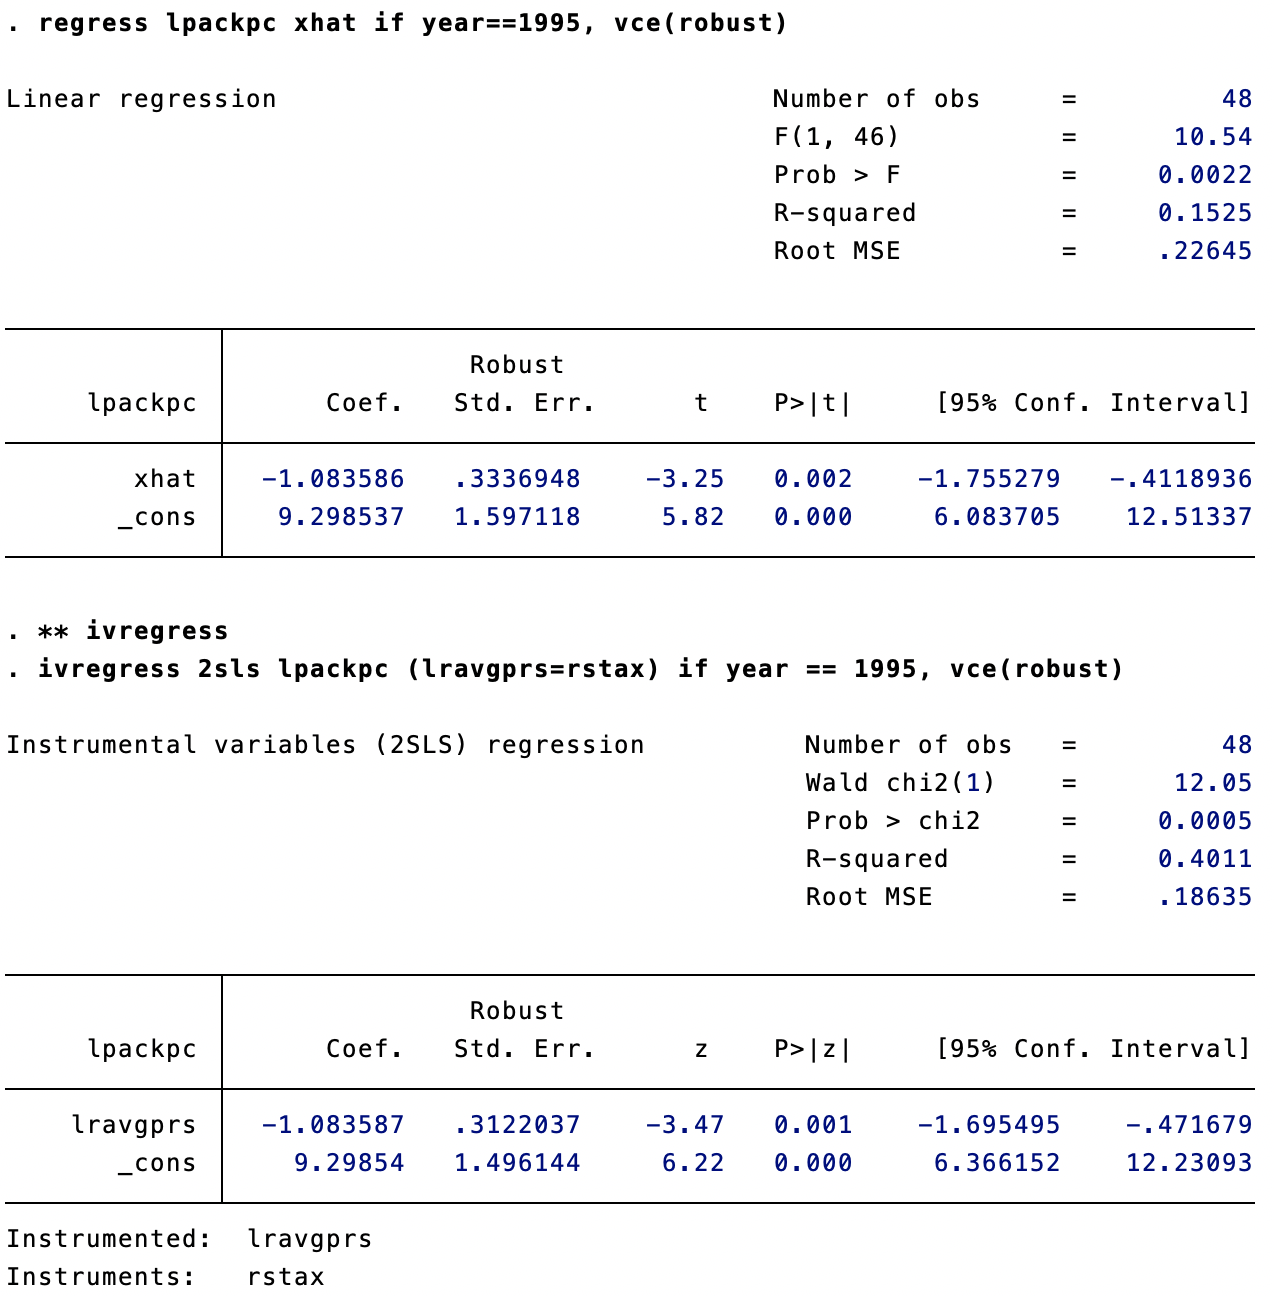
\includegraphics[width=0.8\textwidth,keepaspectratio]{ivregress.png}
\end{figure}
Notice that the standard errors are different. Therefore, if you want to work with correct standard errors, you must use \texttt{ivregress 2sls y x1 (x2 = z)} command.
\subsubsection{Covariance method}
Go back to the part where we discussed the exclusion condition. From there, get
\[
cov(Z,Y)=cov(Z,\beta_1X) \implies cov(Z,Y)=\beta_1cov(Z,X)
\]
From this, we can get
\[
\hat{\beta}_1=\frac{cov(Z,Y)}{cov(Z,X)}
\]
where division is possible because we require a relevancy condition ($cov(Z,X)\neq0$)
\subsubsection{Derivations from the reduced form}
This requires some amount of algebra. Denote the two equations as
\begin{gather*}
X=\pi_0+\pi_1Z+v \ (\text{where }cov(Z,v)=0)\\ Y=\gamma_0+\gamma_1Z+w \ (\text{where }cov(Z,w)=0)
\end{gather*}
When you rewrite the first equation in terms of $Z$, you get
\[
Z=\frac{X}{\pi_1}-\frac{\pi_0}{\pi_1}-\frac{v}{\pi_1}
\]
Then plug this into the second equation. Reorganizing this equation, you should get
\[
Y=\left(\gamma_0-\frac{\pi_0\gamma_1}{\pi_1}\right)+\left(\frac{\gamma_1}{\pi_1}\right)X+\left(w-\frac{\gamma_1}{\pi_1}u\right)
\]
What this gets you is that $\beta_1$ from the equation where we had $X$ as independent variable is $\beta_1 = \frac{\gamma_1}{\pi_1}$. This also implies that when $Z$ rises by 1 unit, $X$ exogenously changes by $\pi_1$ units and $Y$ changes by $\gamma_1$ as a result. In other words, 1 unit of exogenous change in $X$ translates to  $\beta_1 = \frac{\gamma_1}{\pi_1}$ units of change in $Y$. \par\medskip



\subsection{Properties of IV estimators}
Note that the IV estimator can be written in terms of the ratios of the two covariances. In sample analogs, it is written as
\[
\hat{\beta}_{1,\text{TSLS}}=\frac{s_{zy}}{s_{zx}}=\frac{\frac{1}{n}\sum_{i=1}^n(Z_i-\bar{Z})(Y_i-\bar{Y})}{\frac{1}{n}\sum_{i=1}^n(Z_i-\bar{Z})(X_i-\bar{X})}
\]
Note that $\frac{1}{n}\sum_{i=1}^n(Z_i-\bar{Z})(Y_i-\bar{Y})$ is not an unbiased estimator for the covariance of $Z,Y$ (and similar for $\frac{1}{n}\sum_{i=1}^n(Z_i-\bar{Z})(X_i-\bar{X})$) If you have large samples, however, then $\frac{1}{n}\sum_{i=1}^n(Z_i-\bar{Z})(Y_i-\bar{Y}$) is a \textbf{consistent} for covariance of $Z,Y$\footnote{However, $\frac{1}{n-1}\sum_{i=1}^n(Z_i-\bar{Z})(Y_i-\bar{Y})$ is unbiased. For more information refer to \url{https://math.stackexchange.com/questions/2019122/unbiased-estimate-of-the-covariance}}. In mathematical terms, $s_{YZ}\xrightarrow{p} cov(Y,Z),  s_{XZ}\xrightarrow{p} cov(X,Z)$. With these properties, we can say that the IV estimator of $\beta_1$, which is $\hat{\beta}_{1,\text{TSLS}}$ is a consistent estimator for the true $\beta_1$ \par\medskip

The notion of IV estimation does not change much even in multiple regression settings. Suppose that we have
\[
Y_i = \beta_0 + \beta_1X_{1i} +...+ \beta_kX_{ki} + \delta_1W_{1i}+...+\delta_lW_{li}+u_i 
\]
where $X$ variables are endogenous and $W$ variables are exogenous. Assume that we have found a total of $m$ (not necessarily, equal. We'll save the discussion to overidentification test) variables that could qualify as IVs. Additionally, IV regression requires these assumptions 
\begin{description}
\item[\textbf{IV1}] $E[u_i|W_{1i},...,W_{li}]=0$ (At least for exogenous variables, this is satisfied)
\item[\textbf{IV2}] $(Y_i,X_{1i},..,X_{ki},W_{1i},..,W_{li},Z_{1i},...,Z_{mi})$ are IID
\item[\textbf{IV3}] The $Y,X,W,Z$ variables all have nonzero finite 4th moments
\item[\textbf{IV4}] The instruments are valid. That is $cov(Z_{ji},u_i)=0$ for all $j=1,...,m$ and relevancy conditions are satisfied for all $Z$'s. 
\end{description}
\subsection{Identification issues}
In a general sense, a parameter is \textbf{identified} if different values of the parameter produce different distributions of the data. In other words, there is a one-to-one matching of the parameters and the distributions. For instance, A normal distribution with mean $\mu$ and variance $\sigma^2$ is identified because different values of $\mu, \sigma^2$ produce different distributions. If it is the case that the same distribution can be obtained from different parameter values, we say that the parameters are not identified. \par\medskip

In the context of IV's, the parameters we are interested are coefficients for the independent variables. This depends on how much instrument variables ($m$ in the previous section) we have relative to the endogenous variables ($k$). There are three possible cases
\begin{description}
\item[\textbf{Just-identified}]: When $m=k$. There are just enough instruments to identify $k$ endogenous variables
\item[\textbf{Overidentified}] When $m>k$. There are more than enough instruments. We later test whether the instruments are valid using \textbf{overidentification test}.
\item[\textbf{Underidentified}] When $m<k$. There are not enough instruments. The coefficients for $X$'s will not be identified 
\end{description}
So the key takeaway here so far is that when you are using IV, you need at least as much instrumental variables as the number of endogenous regressors you have. Now the issue is having too much IV bad? That depends on the answer we get from the overidentification test.\par\medskip
\textbf{Overidentification test} applies to the case where $m>k$ and aims to test whether the instrument variables we found are valid. To nail this idea more clearly, suppose that we only have one independent variable that is also endogenous  -$X_i$. Also suppose that we have two instrumental variables - $Z_{1i}, Z_{2i}$. Now, we run two two-stage least squares regression with each one of the instrumental variables. The estimates for the coefficient for $X$ are 
\[
\hat{\beta}_{Z_1}=\frac{cov(Z_1,Y)}{cov(Z_1,X)}, \ \hat{\beta}_{Z_2}=\frac{cov(Z_2,Y)}{cov(Z_2,X)}
\]
The numbers look different, although both $\hat{\beta}$'s are suppose to be the same coefficient estimating impact of $X_1$ on $Y$. The overidentification test checks whether the differences between $\hat{\beta}_{Z_1}, \hat{\beta}_{Z_2}$ are large. If the two estimates are similar in the sense that the sample analogs of both $\frac{cov(Z_1,Y)}{cov(Z_1,X)}$ and $\frac{cov(Z_2,Y)}{cov(Z_2,X)}$ converge to the same thing in probability, we don't really have to worry. If they converge to something different, then we may have problem with either one or potentially both instrumental variables. Therefore, the takeaway from overidentification test is that it checks whether there exists a faulty IV variable in the case where we found too many candidates for instrumental variables. 
\end{document}


%%%%%%%%%%%%%%%%%%
\chapter{Economics of Experiments}
\section{Motivation}
In previous chapters, we have learned that one way to control for many internal validity threats - such as selection bias, omitted variable bias - is an \textbf{ideal randomized controlled experiments}. This is where you categorize some individuals under treatment group and controlled group and run various tests as if you are in a laboratory experiment. While there are some degrees of randomized controlled experiments (not necessarily ideal, in the sense that subjects were not brought to the lab), this is difficult to conduct, due to logistical, financial, and ethical reasons. The alternative is to use a \textbf{quasi-experiment} or \textbf{natural experiments}. This is where there exists an exogenous event (like natural disasters, policy change etc) that affect some groups of the population differently than the others.  To see the impact of the said event, we need to be able to compared the affected group (treatment) and the unaffected group (controlled) across different time periods. \par\medskip

So what is the value in studying experiments? For one thing, they provide a conceptual benchmark for assessing observational studies. In particular, experiment is one of the ways to see how economic theories can be applied in reality. More importantly, unlike surveys, they are free from various internal validity threats. Surveys suffer from selection bias - if people don't respond to surveys anymore and they are different from those who respond, we fail to obtain a representative sample. However, experiments suffer from their own validity threats. 
\begin{mdframed}[backgroundcolor =blue!10]
\textbf{Example of randomized controlled experiments}
\begin{itemize}
\item \textit{What are the barriers to technology adoption?} This is from a research of Prof. Eric Verhoogen of Columbia (with some co-authors)\footnote{\scriptsize{Atkin, D., A. Chaudhry, S. Chaudry, A. K. Khandelwal, E. Verhoogen (2017), Organizational Barriers to Technology Adoption: Evidence from Soccer-Ball Producers in Pakistan, \textit{The Quarterly Journal of Economics}, 132(3): 1101–1164}}. This team of researchers developed a new cutting technology that reduces waste of primary raw material involved in making soccer balls. Initially it gave a random subset of Pakistani producers an access to the technology. The take-up rate was very low, for surprising reasons. Then, they noticed that the employees get paid according to the number of soccer balls made, not taking into account the waste of resources involved. Since the new technology slowed them down initially, employees were reluctant to accept new technology. Then, the team conducted another experiment within the firms that had the access to the technology. Within each firm, one cutter and one printer received a lump-sum payment equivalent to monthly earnings. However, there is a string attached - each worker must be able to use the technology in presence of their owner. As a result, employees accepted the new technology more. \par\medskip
\noindent
\end{itemize}
\textbf{Example of natural experiments}
\begin{itemize}
\item \textit{What are the impacts of prenatal exposure to radioactive fallout?} This is from Prof. Douglas Almond and Prof. Lena Edlund's research\footnote{\scriptsize{D. Almond, L. Edlund, M. Palme (2009), Chernobyl's Subclinical Legacy: Prenatal Exposure to Radioactive Fallout and School Outcomes in Sweden, \textit{The Quarterly Journal of Economics}, 124(4): 1729–1772}}. They notice that different regions in Sweden were exposed to different levels of radioactive fallout as a result of Chernobyl disaster (the levels of fallout were generally considered physically harmless). Using this exogenous variation in radioactive fallout, they see whether exposure to such fallout has impacts on childhood cognitive abilities. The experiment reveals that those exposed more to the fallout performed worse in secondary school, mathematics in particular.  
\end{itemize}
\end{mdframed} \par\medskip

\section{Potential outcomes framework}
In class, we have discussed the possibility that the effect of treatment can differ depending on an individual (and hence the $\beta_{1i}$) notation. This is more realistic but also more difficult to address. So I will start by assuming that the treatment effect is identical for everyone (\textbf{constant treatment effect} assumption).\par\medskip
The framework, in its most simplest form, is as follows: Let $Y_{i,t}$ be the \textbf{observed} outcome variable for individual $i$ at time $t$, $X_{it}$ be the treatment variable: It is $1$ if individual $i$ is treated and $0$ if otherwise. In equation form, we can write
\[
Y_{it}=\beta_0+\beta_1X_{it}+u_{it}
\]
\par\medskip
Now we define a \textbf{potential outcome framework}, which is a key in understanding how to identify treatment effects in regressions.  Let $Y_{it}(0)$ denote a potential outcome if subject $i$ is not treated at time $t$ and $Y_{it}(1)$ be the same if $i$ is treated. Then $Y_{it}$, the observed outcome for individual $i$ at time $t$, can be split into
\[
\begin{aligned}
Y_{it} & = Y_{it}(1)X_{it}+Y_{it}(0)(1-X_{it})\\
&=Y_{it}(0)+(Y_{it}(1)-Y_{it}(0))X_{it} \\
\end{aligned}
\] 
\par\medskip
This equation captures so many things. For one, we always see what $Y_{it}$ is whether $i$ is treated or not. However, we can only observe at most one of $Y_{it}(1)$ and $Y_{it}(0)$. This is because the very same individual $i$ cannot be treated and untreated at the same time period $t$. This leads to what we call \textbf{fundamental problem of missing data}. For us to make any rigorous statements about the treatment effect, we need to be sure about what the missing outcome looks like. This is where perfect randomization, randomization conditional on observables, using instrumental variables on treatment variable $X_{it}$ comes in.
\par\medskip
Second, this framework (the second line in the equation above) gives hints as to how we can identify the treatment effect in a regression. $\beta_1$ itself would be enough to identify treatment effects. Even if we allow treatment effects to differ, we can obtain \textbf{average treatment effect}, which can be written as
\[
ATE = E[Y_{it}(1)-Y_{it}(0)]=\frac{1}{N}\sum_{i=1}^N(Y_{it}(1)-Y_{it}(0))
\]
which is related to the terms in front of the $X_{it}$ variable. It gives us the hint that ATE can be obtained from estimating the right coefficient in the regression. 
\section{Average treatment effect under perfect randomization}
We will now derive the average treatment effect in a regression. To start with a simple thought experiment, we will assume that the experiment is \textbf{perfectly randomized} - that the treated individuals and controlled individuals are identical except for treatment status, or that $E[u_{it}|X_{it}]=0$ for all possible $X_{it}$ values. In addition, let's assume constant treatment effect for now. Let's use this regression framework along with the potential outcome framework:
\[
Y_{it} = \beta_0 + \beta_1 X_{it}+u_{it}
\] 
We now derive the expected value of $Y_{it}$ separately for the treated and controlled individuals. For the controlled ($X_{it}=0$, so that $Y_{it}=Y_{it}(0)$):
\[
E[Y_{it}|X_{it}=0]=E[Y_{it}(0)]=\beta_0
\]
and for the treated, ($X_{it}=1$, so that $Y_{it}=Y_{it}(1)$)
\[
E[Y_{it}|X_{it}=1]=E[Y_{it}(1)]=\beta_0+\beta_1
\]
Then, the average treatment effect can be characterized as
\[
ATE = E[Y_{it}(1)-Y_{it}(0)]=(\beta_0+\beta_1)-\beta_0=\beta_1
\]
where subtraction among $E[Y_{it}|X_{it}=1]$ and $E[Y_{it}|X_{it}=0]$ is possible since we are assuming perfect randomization. So under the current circumstances, identifying the average treatment effect is equivalent to obtaining the $\beta_1$ coefficient through an OLS process.
\par\medskip
Even if we allow the treatment effect to differ across different individuals, the story is not too different. Define
\[
\beta_{1i}= Y_{it}(1)-Y_{it}(0)
\]
and let $\beta_1=E[\beta_{1i}]$. Here, $\beta_{1i}$ refers to a (raw) treatment effect for an individual $i$ and $\beta_1$ would be the average of all $\beta_{1i}$'s. The potential outcome framework can be formally written as
\[
\begin{aligned}
Y_i & = Y_i(1)X_i+Y_i(0)(1-X_i)\\
&=Y_i(0)+(Y_i(1)-Y_i(0))X_i \\
&=E[Y_i(0)]+(Y_i(1)-Y_i(0))X_i+Y_i(0)-E[Y_i(0)]\\
&=\beta_0+\beta_{1i}X_i+u_i   \\
\end{aligned} 
\]
Here, we will take it a little bit further to write it in an equation involving $\beta_1$. That will be possible by
\[
Y_i = \beta_0 + \beta_1X_i+\underbrace{(\beta_{1i}-\beta_1)X_i+u_i}_{=v_i}
\]
Here, as long as we have perfect randomization, even $E[v_i|X_i]=0$ will hold. you can see that by
\[
\begin{aligned}
E[v_i|X_i]&=E[(\beta_{1i}-\beta_1)X_i+u_i|X_i]\\
&=E[(\beta_{1i}-\beta_1)X_i|X_i]+E[u_i|X_i]\\
&=E[(\beta_{1i}-\beta_1)|X_i]X_i+E[u_i|X_i]\\
&=0\\
\end{aligned}
\]
Thus, with perfect randomization, OLS gives an unbiased estimate of the average treatment effect, whether we assume constant treatment effects or not. 
\section{Validity threats}
However, having a perfectly randomized sample is very bold assumption and a rare circumstance. Like in general cases, there are many threats to the validity of our estimation results. To start with, we cannot automatically subtract $E[Y_{it}|X_{it}=1]$ and $E[Y_{it}|X_{it}=0]$ under \textbf{imperfect randomization}. Moreover, if the \textbf{attrition rate is nonrandom} - if it differs by a treatment status - we end up with a biased estimate of the treatment effect. In terms of experimental procedure, \textbf{failure to comply to experiment protocol} and other \textbf{experimental effects} that rises through peculiar behaviors of the experimental and the experiment subject could also serve as a validity threat. Additionally, constant treatment effect assumption that we have imposed on ourselves may not be accurate. There are external validity threats when the sample is not representative, is not replicable in other settings, and the results may have general equilibrium effects.
\par\medskip
Some ways to address these problems are as follows: If the treated and the controlled differ in some observed characteristics, we can simply include control variables $Z_{it}$.  In that case, we would be observing the average treatment effect conditional on the combination of values observed through $Z_{it}$. This would also allow us to identify treatment effects for people with different treatment effects as well. 
\par\medskip
There is also an instrumental variable approach: If there exists a $Z_{it}$ variable that influences the treatment status $X_{it}$ and uncorrelated with $u_{it}$, we can use $Z_{it}$ to instrument $X_{it}$ and run 2SLS regression. The interpretation becomes slightly different, however. The predicted value of $X_{it}$ used in the second stage represents the probability of being treated as according to $Z_{it}$. Therefore, 2SLS estimation estimates the causal effect for those whose value of $X_{it}$ is influenced by $Z_{it}$ and puts higher weight on those who is more likely to enter treatment. In effect, what we are doing is to measure the treatment effect `localized' for those whose probability of treatment is most influenced by $X_{it}$ with $Z_{it}$ as an instrument. This is what \textbf{localized average treatment effect} (LATE) is about.
\par\medskip
So how do you use IV in an experimental framework? Let $Z_{it}$ be an instrument for $X_{it}$. Then the usual two stage least squares method can be applied in this manner
\begin{gather*}
X_{it} = \pi_0+\pi_{1i}Z_{it}+e_{it} \ \text{(First stage)}\\
Y_{it} = \beta_0+\beta_{1i}X_{it}+u_{it} \ \text{(Equation of interst)}
\end{gather*}
When we are at the first stage, we can obtain predicted $\hat{X}_{it}=\hat{\pi_0}+\hat{\pi}_{1i}X_{it}$. Given that $X_{it}$ is binary, (recall from linear probabilities model), the first stage gets us the predicted probability of being treated. As we did with the typical two stage least squares, we put $\hat{X}_{it}$ in place of $X_{it}$ in the equation of interest. Therefore, it puts more weight on those that are likely to be treated. Then it allows us to measure the causal effect for those whose predicted probability of treatment is heavily influenced by $Z_{it}$ - this is called \textbf{local average treatment effect}. If $\beta_{1i}, \pi_{1i}$ are independent of $(u_{it},v_{it}.Z_{it})$, $E(\pi_{1i})\neq0$, then we can get that
\[
\hat{\beta}_{1}\xrightarrow{p}\frac{E(\beta_{1i}\pi_{1i})}{E(\pi_{1i})} \ \text{(Refer to appendix 13.2)}
\]
Using the fact that $E(\beta_{1i}\pi_{1i})=E(\beta_{1i})E(\pi_{1i})+cov(\beta_{1i},\pi_{1i})$, $\hat{\beta}_1$ can be written as 
\[
\hat{\beta}_{1}\xrightarrow{p} E[\beta_{1i}]+\frac{cov(\beta_{1i},\pi_{1i})}{E(\pi_{1i})} = \beta_1+\frac{cov(\beta_{1i},\pi_{1i})}{E(\pi_{1i})}
\]
In this setting, treatment effect is large for individuals for whom the effect of the instrument is large.
\par\medskip

\section{Some words on Diff-in-Diffs and RD}
The idea in using the \textbf{difference-in-difference}, (hereafter DD) estimator is to see the differences in the pre- and post-treatment outcomes for $Y$ for treatment and control groups. Specifically, it estimates the treatment effect as
\[
\hat{\beta}_1^{DD}=[\bar{Y}_{\text{treat,after}}-\bar{Y}_{\text{treat,before}}]-[\bar{Y}_{\text{control,after}}-\bar{Y}_{\text{control,before}}]
\]\par\medskip
In a regression form, what we can get is as follows (Assume away $W_i$'s for the moment). Suppose we have two time periods, one for before treatment and the other for after treatment. We can write
\[
\Delta Y_i=(Y_{i,\text{after}}-Y_{i,\text{before}}) = \beta_0+\beta_1X_i+u_i
\]
For those who are not treated, $E[\Delta Y_i|X_i=0]=\beta_0$. For those treated, $E[\Delta Y_i|X_i=1]=\beta_0+\beta_1$. These two parameters represent the `difference' within treatment and control groups. By taking the `difference' between treatment and control groups, we are left with $\beta_1$. In other words
\[
\beta_1 = E[\Delta Y_i|X_i=1]-E[\Delta Y_i|X_i=0]
\]
So by taking the 'difference' (between treatment and control groups) of the 'difference' (changes over time within each group), we get the DD estimator (and this is where DD estimator gets its name). \par\medskip
The following picture should make things clear. In the following figure, $T=1$ indicates the treatment group, $T=0$ is the control group

\begin{figure}[H]
\centering 
\caption{DD estimator}
\begin{subfigure}[b]{.4\textwidth}
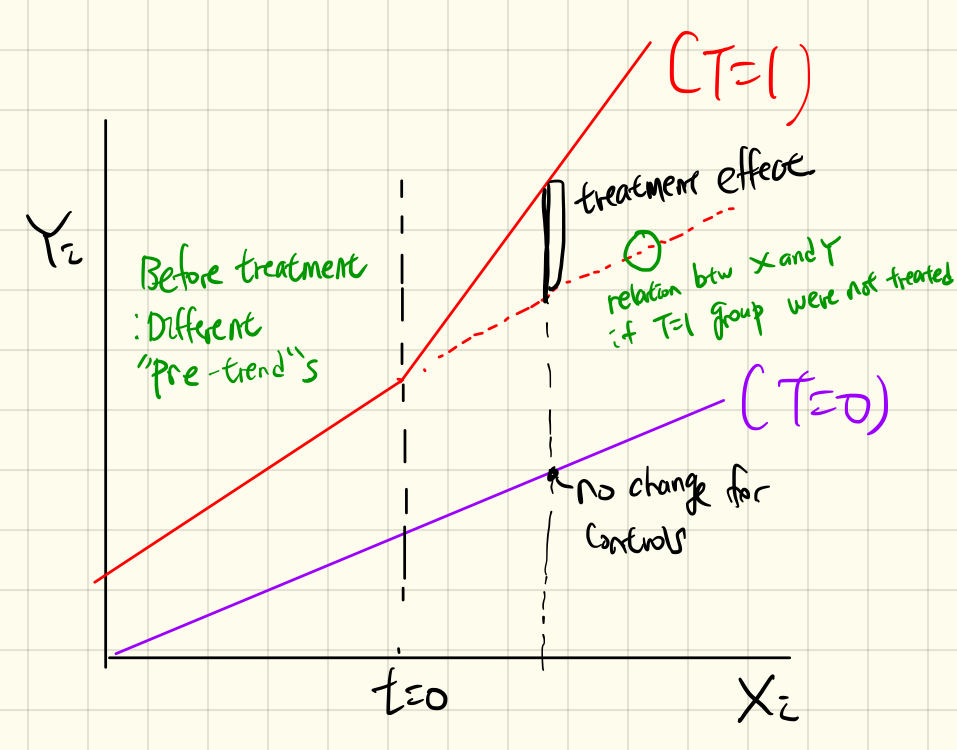
\includegraphics[width=\textwidth]{fig1_1.png}
\caption{No change in control group}
\end{subfigure}
\begin{subfigure}[b]{.4\textwidth}
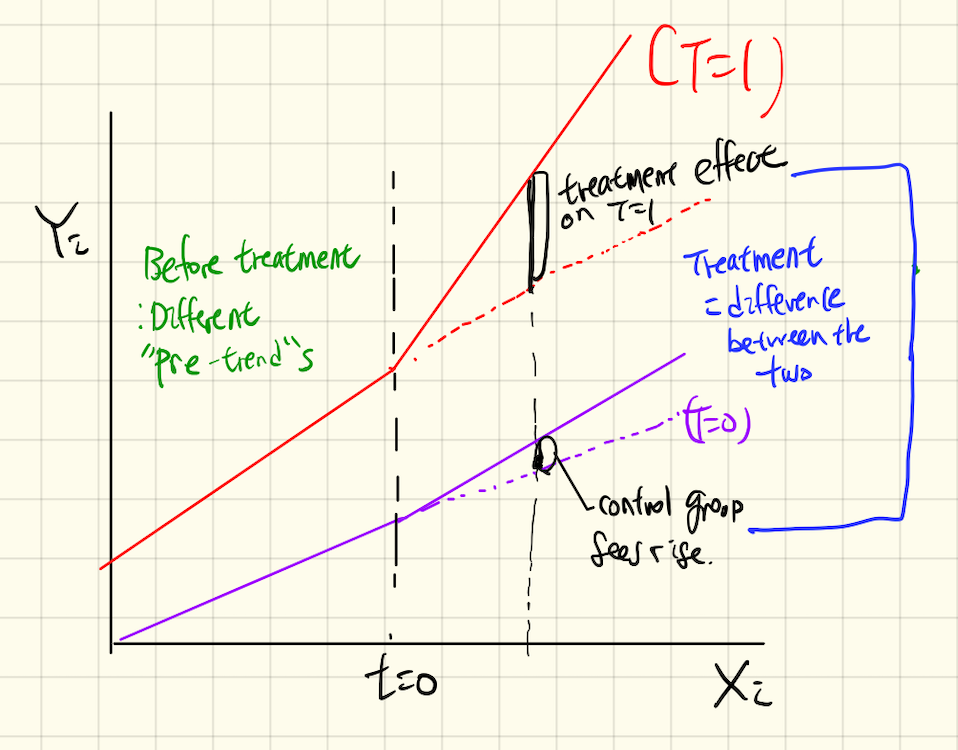
\includegraphics[width=\textwidth]{fig1_2.png}
\caption{Some change in control group}
\end{subfigure}
\end{figure}
In words, the treatment effect measured by the DD estimator is the treatment effect on treated groups \textit{on top of} effect on control groups. 
\par\medskip
\textbf{Regression discontinuity} design (or RD) applies to the case where the treatment status depends on whether individual $i$ has passed a threshold. Suppose that there is a variable $T_i$, like a test score, for instance. Let's assume that there exists a program for gifted students that only accept those whose test score is higher than 90. In this case, $X_i=1$ iff $T_i>90$ and $X_i=0$ if otherwise. In equation,
\[
Y_i  = \beta_0 + \beta_1X_i+u_i
\] 
and the following figure captures the treatment effect in an RD setup.
\begin{figure}[H]
\centering 
\caption{RD treatment effects}
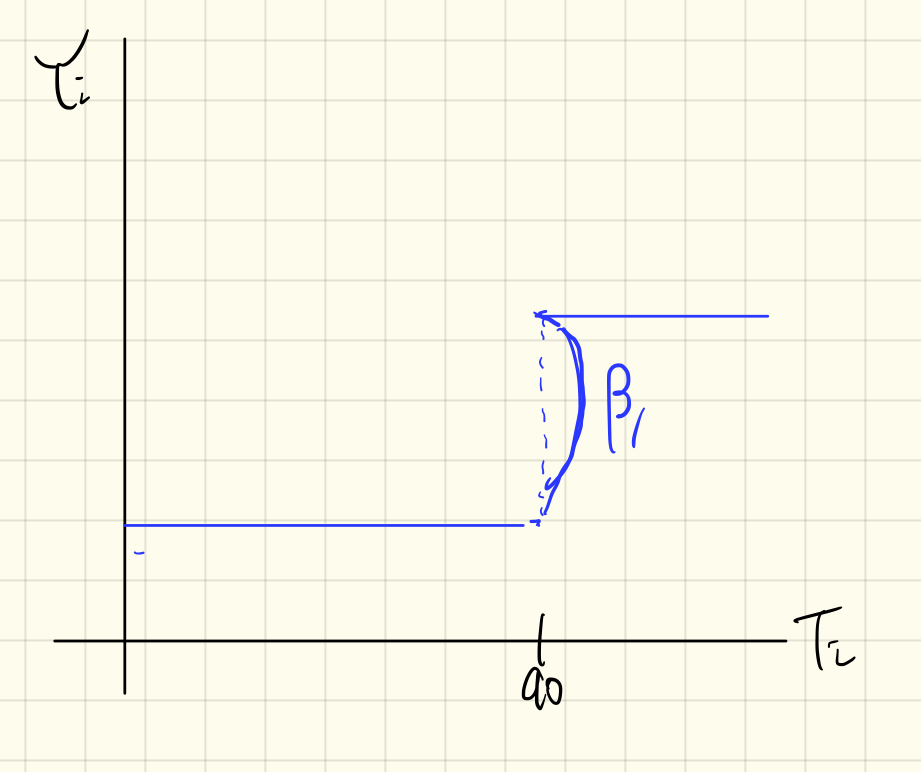
\includegraphics[width=0.4\textwidth]{fig2.png}
\end{figure}
For those not in the program, $E[Y_i|X_i=0]=\beta_0$ and $E[Y_i|X_i=1]=\beta_0+\beta_1$. This implies that if the direct effect of $T$ on $Y$ is continuous in the absence of the treatment, the effect of treatment should show up as a jump of size $\beta_1$ at the threshold value of $T_i$, 90 in our case. Similar to what we have in our figure

\par\medskip
To conduct RD rigorously, many things should be satisfied. Ideally, RD is most accurate in settings where subjects are not different in other traits (especially if we are including control variables $W_i$). In order to achieve this, we usually limit the subjects to those around certain bandwidth of the cutoff value of $T_i$. Therefore, it may induce a loss of sample issue. (This is actually an advanced topic)
\par\medskip
For now, I assumed that everyone whose $T_i>90$ is accepted. This is what is called \textbf{sharp RD}. However, this may not always be the case in reality. There might be exceptions - those whose test score are higher than 90 may not be part of the program and those whose score is under 90 might be part of the program. If this is the case and we carry out an RD here, we are conducting a \textbf{fuzzy RD}. The estimation in the case of fuzzy RD is tricky and quite advanced. So the takeaway here is that the accuracy of RD is susceptible to the compliance (of the program) issue. If the subjects are not fully complaint to the intentions of the program, accuracy of the RD is not fully guaranteed.  



\documentclass[12pt]{article}
\usepackage{geometry}
\usepackage{amsmath}
\usepackage{amssymb}
\usepackage{enumitem}
\usepackage{fancyhdr}
\usepackage{framed}
\usepackage{tikz}
%\usepackage{charter}
\usepackage{mathpazo}
%\usepackage{newcent}
\usepackage{indentfirst}
\usepackage{booktabs}
\usepackage{graphicx}
\usepackage{float}
\usepackage{makecell}
\usepackage{xcolor}
\usepackage{mdframed}
\usetikzlibrary{trees}
\pagestyle{fancy}
\usepackage{amsthm}
\theoremstyle{definition}
\newtheorem{definition}{Definition}[section]
\theoremstyle{property}
\newtheorem{property}{Property}[section]
\theoremstyle{assumption}
\newtheorem{assumption}{Assumption}[section]
\theoremstyle{example}
\newtheorem{example}{Example}[section]
\theoremstyle{comment}
\newtheorem{comment}{Comment}[section]
\newtheorem{theorem}{Theorem}[section]
\newtheorem{corollary}{Corollary}[theorem]
\newtheorem{lemma}[theorem]{Lemma}
\usepackage{lastpage}
\usepackage{wrapfig}
\usepackage{hyperref}
\usepackage{subcaption}
\usepackage{setspace}
\hypersetup{
colorlinks=true,
linkcolor=black,
filecolor=green, 
urlcolor=blue,
}
\newcommand{\ROM}[1]
    {\MakeUppercase{\romannumeral #1}}
\fancyhead[L]{Econometrics \ROM{2}: Recitation 12 }%change each reci
\fancyhead[R]{Spring 2020}
\fancyfoot[C]{\thepage \hspace{1pt} / \pageref{LastPage}}

\fancypagestyle{firstpage}{%
\fancyhf{}%
\renewcommand{\headrulewidth}{0mm}%
  \fancyfoot[C]{\thepage \hspace{1pt} / \pageref{LastPage}}
}

\usepackage{wrapfig}

\lhead{Introduction to Econometrics}

\rhead{Recitation 11}


\title{\Large{Introduction to Econometrics: Recitation 11}}

\begin{document}
\linespread{1.25}
\author{Seung-hun Lee}
\date{}
\maketitle
%%%%%%%%%%%%%%%%%%

\section{Big Data}
Big data can mean so many things: it can simply mean data with large observations or large number of control variables. In general instances, atypical data such as text data, and satellite imagery are referred to as big data. In this class, we focus on the instance where there are many control variables, specifically on what to do if there are many control variables relative to the number of observations. Additionally, we focus on trying to get the best way to predict a result that is currently not in the dataset.
\par\medskip 
\subsection{Prediction with many $X$'s: Why we don't want too many $X$'s}
In this section, we will focus on the issue of \textbf{shrinkage}. I will introduce Ridge estimation, LASSO estimation, and principal component method. Before introducing these models, I will talk about the regression framework that will be used throughout the discussion
\[
Y_{i}^*=\beta_1X_{1i}^*+....+\beta_kX_{ki}^*+u_i^*
\]
where $X_{1i}^*$ is the ``standardized" version of $X_{1i}$'s, defined as
\[
X_{1i}^*=\frac{X_{1i}-\bar{X}_1}{\sigma_{X_{1}}}
\]
and we define $Y^*_i$ as $Y_{i}-\bar{Y}$ - the ``demeaned" version. Note that we CANNOT have a constant term $\beta_0$ here because if we demean $\beta_0$, which is the same for all $i$'s, they vanish. 
\par\medskip
We then define the mean squared prediction error, or MSPE as the expected value of the squared error made by predicting $Y$ for an observation not in the dataset. In maths, 
\[
MSPE= E[Y^{OS}-\hat{Y}^{OS}]^2
\]
where the $\hat{Y}^{OS}$ is obtained from the coefficients of $\beta$'s made from the in-sample prediction
\[
\hat{Y}_i^{OS}=\hat{\beta}_1X_{1i}^{OS}+ ... +\hat{\beta}_kX_{ki}^{OS}
\]
and the $Y^{OS}$ is the realized value of $Y$ outside of the sample
\[
Y_i^{OS}=\beta_1X_{1i}^{OS}+ ... +\beta_kX_{ki}^{OS}+u_i^{OS}
\]
With these notations, we can define the prediction error as
\[
Y_i^{OS}-\hat{Y}_i^{OS}=(\beta_1-\hat{\beta}_1)X^{OS}_{1i}+...+(\beta_k-\hat{\beta}_k)X^{OS}_{ki}+u_i^{OS}
\]
Define $\sigma_u^2=E[u_i^{OS}]^2$, then we can write MSPE as
\[
MSPE=\sigma_u^2+ E[(\beta_1-\hat{\beta}_1)X^{OS}_{1i}+...+(\beta_k-\hat{\beta}_k)X^{OS}_{ki}]
\]
Ideally, the smallest possible MSPE would be $\sigma_u^2$, referred to as the \textbf{oracle prediction}. Which happens if your predicted $\hat{\beta}$'s match the actual $\beta$. Unfortunately, we cannot predict $\beta$'s perfectly. and the more predictors we have, we generally end up having larger MSPE. As such having a large set of $X$'s will not be a good idea (Thus, the \textbf{problem of many predictors}). This is where Ridge, LASSO, and Principal Component method comes in.

\subsection{Big data methods}
The goal here is to find other estimators that does not increase the MSPE compared to the rate in which the same rises in OLS estimators. The idea here is to reduce the $\sigma_u^2$, the variance from the residual sums of squares, at the expense of introducing a small bit of bias. We do this by providing a penalty for having a model with large number of regressors (what we formally call `shrinkage'). All of the methods I introduced above involve these tricks. 
\subsection{Ridge regression}
The Ridge regression minimizes a `penalized' sum squared of residuals in the following sense
\[
\hat{\beta}_{Ridge}=\arg\min_{\beta_1,..,\beta_k}\left[ \sum_{i=1}^n(Y_i - \beta_1X_{1i}-....-\beta_kX_{ki})^2 + \lambda_{Ridge}\sum_{j=1}^k\beta_j^2\right]
\]
Here, the last term on the right hand side is the penalty we are introducing. Note that for any term in which $\beta_j$ is not zero, the penalty term is also nonzero. Also note that we are introducing some degree of bias (compared to OLS). However, the gain is that the variance term $\sigma_u^2$ will be reduced. Lastly, you need to capture that the variance and the bias that determines the MSPE moves in a trade-off relation - If you want to decrease one component, you increase the other (but not at a 1-for-1 rate). The Ridge estimator that comes from here minimizes MSPE by working through reducing the variance term to the extent that the bias term does not rise too drastically. 

\subsection{LASSO regression}
LASSO regression also minimizes a penalized sum squared residuals. The difference is that the penalty term takes a different form: 
\[
\hat{\beta}_{LASSO}=\arg\min_{\beta_1,...,\beta_k}\left[ \sum_{i=1}^n(Y_i - \beta_1X_{1i}-....-\beta_kX_{ki})^2 + \lambda_{LASSO}\sum_{j=1}^k |\beta_j|\right]
\]
In essence, the idea is similar with the Ridge regression - you find an estimator that minimizes MSPE by reducing $\sigma_u^2$ at the expense of some amount of increase in the bias. 
\par\medskip
The difference between the two lies in the degree of shrinkage. The difference is stark when the OLS estimates are virtually close to zero. When the OLS estimates are small, the LASSO shrinks those estimates all the way to 0. While Ridge also shrinks those coefficients close to 0, they do not exactly set them to 0. 
\subsection{Principal component}
Say that you have a giant $k$ number of regressors. In the principal component method, you are using a linear combination of some subset of $k$ variables. At the end, you end up using $p<k$ number of regressors and effectively `collapsing' the model to a smaller dimension. 
\par\medskip
So how do you determine the right linear combinations? For a two-variable case, the linear combination looks something like
\[
aX_1 + bX_2
\]
where $a,b$ are some real numbers. The optimal value of $a$ and $b$ is determined by
\[
\max var(aX_1+bX_2)\  \text{s.t.}\ a^2+b^2=1
\]
Note that we want to solve the \textit{maximization} problem in this case as we want the $X$'s to explain more of the variation that we observe in the data. You can understand $a^2+b^2=1$ as a regularization method. 
\par\medskip
So for a general case, you would be solving the following problem to get the $j$'th principal component $PC_j$
\[
\max var\left(\sum_{i=1}^Ka_{ji}X_i\right)\  \text{s.t.}\ \sum_{i=1}^ka_{ji}^2=1
\]
with another condition being that $corr(PC_j,PC_{j-1})=0$. This additional condition is here because we want to minimize the overlapping amount of information across different principal components.
\par\medskip
So we still need to determine how many principal component to use. Scree plot gives you an idea about how much each new principal component adds to the variation that is explained by additional principal component. However, this does not give rigorous cutoff. For formal approach, $m$-fold cross validation approach can be used. You split the sample into $m$ subsets of equal size. Then, one of them becomes your `test' sample and the rest becomes an out-sample. You will derive a first estimate of MSPE. Repeat this for each of the $m$ subsets until you get $m$ estimates of MSPE. The right number of  principal components minimizes the averages of these MSPEs. Note that determining the $\lambda$'s in LASSO and Ridge can also be done by using the $m$-fold cross validation. 

\section{Time series estimation}
Now we shift our attention to the \textbf{time series} data, where we collect data on same observational unit $i$ for multiple time periods. Primary uses for time series include forecasting, modeling risks, and analyzing dynamic causal effects. Time series differs from previous models in that errors are likely to be autocorrelated and thus require different ways to calculate the standard error. Moreover, we introduce time lagged variables into the independent variables.
\par\medskip
Some terms need to be cleared out. Let $Y_t$ be the time series data captured at certain period $t$ - GDP, for instance. \textbf{Lags} are characterized as $Y_{t-1}$ and \textbf{leads} are defined as $Y_{t+1}$. You will also be seeing a lot of $\Delta Y_{t}\equiv Y_t-Y_{t-1}$, which is the \textbf{first difference} at time $t$. 
\par\medskip
\subsection{AR and ADL Models}
We first consider the $p$th order \textbf{autoregressive model}, or AR($p$) for short. This class of models refers to any model in which $Y_t$ is regressed against its own lagged values. They take the following form
\[
Y_t = \beta_0+\beta_1Y_{t-1}+...+\beta_pY_{t-p}+u_t \tag{2}
\]
each coefficients in front of $Y_{t-j}, j\in\{1,..,p\}$ indicate whether they are useful for forecasting future values of $Y_t$. To see if they are individually useful for forecasting purposes, we test whether $H_0:\beta_j=0$ against $H_1:\beta_j\neq0$.
\par\medskip
To simply the discussion of the properties of AR($p$) models, we restrict to the case where $p=1$. I first focus on the difference between `predicted' values and the `forecasts'. Predicted values refer to in-sample fitting. Forecasts focus on future values which are out of the sample. Suppose we have data of up to $T$ periods. Suppose we want to predict the value of $Y$ at period $T+1$, which is out of sample. Keeping the following notation in mind would be useful
\begin{itemize}
\item $Y_{T+1}: $ True value of $Y$ at $T+1$
\item $\hat{Y}_{T+1|T}: $ Forecast of $Y_{T+1}$ based on the estimated coefficients obtained from regressing data that we have up to period $T$. That is, $\hat{Y}_{T+1|T}=\hat{\beta}_0+\hat{\beta}_1Y_T$
\item $Y_{T+1|T}: $ Forecast of $Y_{T+1}$ based on the population coefficients up to period $T$. That is, $Y_{T+1|T}=\beta_0+\beta_1Y_T$
\end{itemize}
Then we are ready to define the \textbf{forecast error}. Forecast error refers to how much $\hat{Y}_{T+1|T}$ deviates from the actual $Y_{T+1}$ value, or $Y_{T+1}-\hat{Y}_{T+1|T}$. The best forecast is the one that minimizes the forecast error. 
\par\medskip
We can conduct a time series regression where $Y_{t-j}$ are not the only independent variable. For a better forecast, it makes sense to control for other variables, denoted as $X$, that captures the movement of $Y$. Such models are called \textbf{autoregressive distributed lag model}, or ADL($p,q$) for short. They have $p$ lags of dependent variable and $q$ lags for $X$ variable. It takes the following form:
\[
Y_t = \beta_0+\beta_1Y_{t-1}+...+\beta_p Y_{t-p} + \delta_1 X_{t-1}+...+\delta_qX_{t-q}+u_t \tag{3}
\]
ADL models are similar in form to AR models, except that we include lagged variables for $X$.
\par\medskip
So what is the right amount of lags for $Y$ and $X$ variables? One way to answer this is to check for the various values of the \textbf{information criteria}. There are two types
\[
\begin{aligned}
AIC:& \ln\left(\frac{SSR(p,q)}{T}\right)+(K)\frac{2}{T}\\
BIC:& \ln\left(\frac{SSR(p,q)}{T}\right)+(K)\frac{\ln{T}}{T}\\
\end{aligned}
\]
where $K=1+p+q$. We want to find the right combination of $(p,q)$ that minimizes the two criteria above. Increasing $p$ and $q$ decreases $SSR(p,q)$ as more of the variation is explained by the right hand side variables. How much it decreases can differ depending on the combination of $p$ and $q$ (Trial and error!). However, any increase in $p$ and $q$ raises the rightmost terms in the above two information criteria. Lastly, BIC usually penalizes complexity higher than AIC since $2<\ln{T}$ as $T\to\infty$. 
\par\medskip
To see whether $X$'s help us predict $Y$, we use the \textbf{Granger causality test}. It is a joint hypothesis test that states, in the null, that none of the $X$'s are a useful predictor above and beyond what is predicted by lagged $Y$'s. In equation (3), the hypotheses can be written as
\[
H_0: \delta_1 = ... = \delta_q=0, \ \ H_1: \lnot H_0
\]
If the null hypothesis is rejected, we say that $X$ \textit{Granger-causes} $Y$. Note that this refers to the idea that $X$ contains information that help us (marginally) predict $Y$ (or the idea of correlation). It does not imply that $X$ causes $Y$, as regression usually captures the idea of causality\footnote{Clive Granger (Nobel Prize in Economics winner at the year 2003), who came up with Granger causality test, argued that causality in economics could be tested for by measuring the ability to predict the future values of a time series using prior values of another time series. However, idea of "true causality" is still being contested and the above statement could fall into  \textit{post hoc ergo propter hoc} fallacy of assuming that one thing preceding another can be used as a proof of causation.  }. 


\subsection{Stationarity}
Ideally, we want the distribution of of time series to be \textbf{stationary}. We say $(Y_{t+1},..,Y_{t+s})$ is stationary if the distribution of $(Y_{t+1},..,Y_{t+s})$ does not depend on $t$. In other words, the distribution of $Y$ does not change over time. This is when we can use an in-sample data for an accurate analysis of prediction and dynamic causal relations. When there is a trend or a break in the movement of the data (or any change in underlying parameters), the data is nonstationary. If the data is nonstationary, we need to detrend the data. 
\par\medskip
A trend is defined as a persistent, long-term movement in the data. There are two types of trends. \textbf{Deterministic trend} is a nonrandom  function of time, ($Y_t = \alpha t^2$). \textbf{Stochastic trend} is random, and time-variant. A random walk defined as $Y_t = Y_{t-1}+u_t$ is a type of stochastic trend. In this particular setting, the best predictor of $Y_{T+1}$ given data at $T$ is $Y_T$ itself. Moreover, we can check that $var(u_t)$ is
\[
Y_t = Y_{t-1}+u_t = Y_{t-2}+u_{t-1}+u_t = ... = Y_0 + u_1 + ... +u_t
\]
If $Y_0=0$,  then assuming $u_t$ has no serial correlation, we get that $var(Y_t)=t\sigma_u^2$. Therefore, $Y_t$ is not stationary. However, if you difference $Y_t$ you will be able to see that the above process is stationary. This is because
\[
\Delta Y_t = Y_{t-1}-Y_{t-1}+u_t = u_t
\]\par\medskip
and $E[\Delta Y_t ]=0$.
\par\medskip
One of the most well-known nonstationary time series is a random walk process. A random walk is equal to AR(1) of $Y_t = \beta_1Y_{t-1}+u_t$ with $\beta_1=1$. Also, for $\beta_1>1$ we have a case where $Y_t$ values blow up and not become stationary. 
\par\medskip
So how do we test for stationarity? Informally, we can always do an `eyeball' test: In a graph, do you see some sort of trend - say upward or downward - across long span of time? For a formal test of stationarity, we need to use a Dickey-Fuller test. We go back to our random walk to find out how. Suppose we have $Y_t = \beta_1 Y_{t-1}+u_t$. After multiple iterations, we can re-write $Y_t$ as
\[
Y_t = \beta_1^T Y_{t-T}+\beta_1^{T-1}u_{t-T+1}+...+\beta_1 u_{t-1}+u_t
\]
If it is the case that $|\beta_1|<1$, then $Y_{t-T}$ has no long term effect. If otherwise, they do. So to check whether the data is stationary, we see if there exists a \textbf{unit root} or not. In a generalized $AR(p)$ setup, we have 
\[
\begin{aligned}
 Y_t&=\beta_0 + \beta_1 Y_{t-1}+ ...+\beta_pY_{t-p}+u_t\\
 &=\beta_0 + \beta_1Y_{t-1}-\beta_2 Y_{t-1}+\beta_2Y_{t-1}+\beta_2 Y_{t-2}+...+\beta_pY_{t-p}+u_t\\
 &=\beta_0 + (\beta_1+\beta_2)Y_{t-1} -\beta_2 \Delta Y_{t-1} - \beta_3Y_{t-2}-\beta_3Y_{t-1}+\beta_3Y_{t-1}+\beta_3Y_{t-2}+\beta_3Y_{t-3}+...\\
 &=\beta_0 + (\beta_1+\beta_2+\beta_3)Y_{t-1}-(\beta_2+\beta_3)\Delta Y_{t-1} - \beta_3\Delta Y_{t-2}+ .. +\beta_pY_{t-p}+u_t
  \\
 &=\beta_0 + (\beta_1+...+\beta_p)Y_{t-1}-(\beta_2+...+\beta_p)\Delta Y_{t-1} - ... - \beta_{p}\Delta Y_{t-p+1}+u_t \\
 \end{aligned}
\]
By further subtracting $Y_{t-1}$ from both sides, we get
\[
\Delta Y_{t} = \beta_0 + (\beta_1 + ,.. +\beta_p-1) Y_{t-1}+ ... +u_t = \beta_0 + \delta Y_{t-1}+ ... +u_t 
\]
where $\delta = \beta_1 + ,.. +\beta_p-1$. To check for stationarity, we set the hypothesis as 
\[
H_0: \delta\geq0 \ (\beta_1+...+\beta_p\geq 1),\ H_1 : \delta<0 
\]
If there is a unit root in the model, then $\delta=0$ and the data is nonstationary. Dickey Fuller test uses this idea to check for the existence of stationarity in the data. In a simple $AR(1)$, this reduces down to
\[
H_0: \beta_1\geq 1,\ H_1 : \beta_1<1 
\]
\par\medskip
Note that the critical value of this test differs depending on whether we are assuming a drift (intercept only) or drift \& time trend (intercept and a term that is a function of $t$).
\par\medskip
Another pattern in which the stationarity can be broken is through a structural break. Assume a ADL(1,1) structure, but that we know when the structural break occurs (e.g. Oil shock and the oil price). Suppose that the shock happens at year $\tau$ Let $D_t(\tau)=1$ if year $t\geq\tau$ and 0 otherwise. Then we write the equation as
\[
Y_t = \beta_0 +\beta_1Y_{t-1}+\delta_1 X_{t-1} + \gamma_1 D_t(\tau)+\gamma_2 D_t(\tau)Y_{t-1}+\gamma_3 D_t(\tau)X_{t-1}+u_t
\]
To check for the existence of a structural break, all we need is a joint hypothesis of the following form:
\[
H_0: \gamma_1 = \gamma_2 = \gamma_3 =0, \ H_1: \lnot H_0
\]
This is the idea behind the \textbf{Chow test}. If the data of the structural break is unknown, we can do a \textbf{Quandt Likelihood Ratio test}, which effectively carries out multiple Chow tests and finds the time point where structural break most likely happened, if it occurred.  
\subsection{Dynamic causal analysis}
We are now interested in whether our independent variable $X$ has cause changes in $Y$ over time. \textbf{Dynamic causal effect} is intended to capture the effect of $X$ on $Y$ over time. To analyze this, \textbf{Distributed lag model} comes in handy. They can be written as
\[
Y_t = \alpha+\beta_0X_t + \beta_1X_{t-1}+...+\beta_pX_{t-p}+u_t
\]
The interpretation of the coefficients are as follows: $\beta_0$ captures the contemporaneous impact of $X$ on $Y$, holding past values of $X$ constant. $\beta_j , j\in[1,p]$ captures the impact of $X$ from $j$ period(s) ago on $Y$, holding $X$ from other periods constant. We can analyze the cumulative effect by summing over multiple $\beta$'s. If we are interested in the effect of $X$ 1 period ago, we can check $\beta_0 + \beta_1$ and so on. Specifically, we can write
\[
\begin{aligned}
Y_t& = \alpha+\beta_0X_t + \beta_1X_{t-1}+u_t\\
&=\alpha +\beta_0 X_t - \beta_0X_{t-1} + \beta_0 X_{t-1} + \beta_1 X_{t-1}+u_t \\
&=\alpha + \beta_0\Delta X_t + (\beta_0 + \beta_1)X_{t-1}+u_t\\
\end{aligned}
\]
\par\medskip
However, for this to be accurately measured, we need following assumptions. 
\begin{itemize}
\item (Sequential) Exogeneity: $E[u_t|X_t, X_{t-1},...,X_1]=0$. Or that error terms should not be correlated with current and past values of $X$
\item Stationarity: $Y$ and $X$ should have stationary distributions and ($Y_t, X_t$) and ($Y_{t-j}, X_{t-j}$) becomes independent as $j$ gets large. 
\item $Y$ and $X$ has nonzero finite moments
\item There is no perfect multicollinearity
\end{itemize}
Key focus is on the first assumption. Sequential exogeneity implies that the error term should not be correlated with independent variables - past and present. If otherwise, the estimates of $\beta$'s will be biased. There is a more stronger assumption that this, called \textbf{strict exogeneity}, that states that the error term should not be correlated with $X$ for not only past and present, but also the future. In the above, setup, sequential exogeneity is sufficient.
\par\medskip
In addition, we need to consider a different type of standard errors. Given that there is a possibility that autocorrelation can exist, we need a standard error that takes into account autocorrelation and heteroskedasticity. This is known as \textbf{heteroskedasticity and autocorrelation consistent} errors (HAC errors). The takeaway is that standard errors in the typical STATA output can be wrong and we need to take a slightly different approach. 


\end{document}

\end{document}
